\section{ALL PLACHOLDER SECTIONS COME HERE}

%\section{Dataset Description}
\label{sec:dataset}

In this section, we describe the three datasets: \moball, \mobcomp, and \mobexpt. 
We use these datasets in our studies that we present in the subsequent sections.

\tbd{Run genDataSetDescription.R to get these numbers} 
The \moball dataset consists of mobile data traffic traces from \tbdv{23} devices that belong to \tbdv{18} users who are volunteers of an IRB approved study. 
This dataset consists of \tbdv{8} iPhones, \tbdv{3} iPads, \tbdv{1} iPodTouch, \tbdv{10} of Android phones, and \tbdv{1} of Android tablet.
We consider an Android device that accesses the Internet by using only \wifi to be a tablet. 
The Android devices used to generate this dataset include the Nexus, Sony, Samsung, and Gsmart brands. 
The users of these devices are spread across France and USA. We observed connections from \tbdv{52} different ISPs.
This dataset consists of \tbdv{171} days of data that was captured on our servers and for each device the number days varies from \tbdv{5} to \tbdv{171} with a median of \tbdv{34} days.  

The \mobcomp dataset consists of data from two users who had three and two devices respectively. 
The three devices that belong to one of the two users consists of a two smart phones and a tablet, while one smartphone and a tablet belong to the second user. 
We use this dataset to compare the behavior of popular apps and to detail the behavior of devices when the device is kept idle. 
The data set consists of \tbdv{number} of days of data from each device and \tbd{number} of days for which data traffic was seen for all the 24 hours. 

The \mobexpt dataset contains the traffic traces from an Android device and an iOS device that were used to perform a controlled experiment on popular application. 
We tested \tbdv{number} of Android applications and \tbdv{number} of iOS application for this study. 
\tbd{How we decided this list}. \tbd{How we performed the test} \tbd{other attributes of this dataset}.

%%% Local Variables: 
%%% mode: latex
%%% TeX-master: "main"
%%% End: 


%%\section{Measurements}
%\label{sec:measurements}

\eat{All the subsections are now sections. We can merge them later}

\section{Network Characteristics of Notification Services}
\label{sec:characterize-os}

Mobile operating systems provide OS level notification services to optimize network usage.
The Apple Push Notification service (APNs) and Google Cloud Messaging (GCM)~\cite{gcm} are used by iOS and Android applications respectively to receive notifications from the Internet.
In this section we show how \platname was used to compare the notification services of iOS and Android, and detailing it behavior in the wild. 

\begin{figure}
\centering
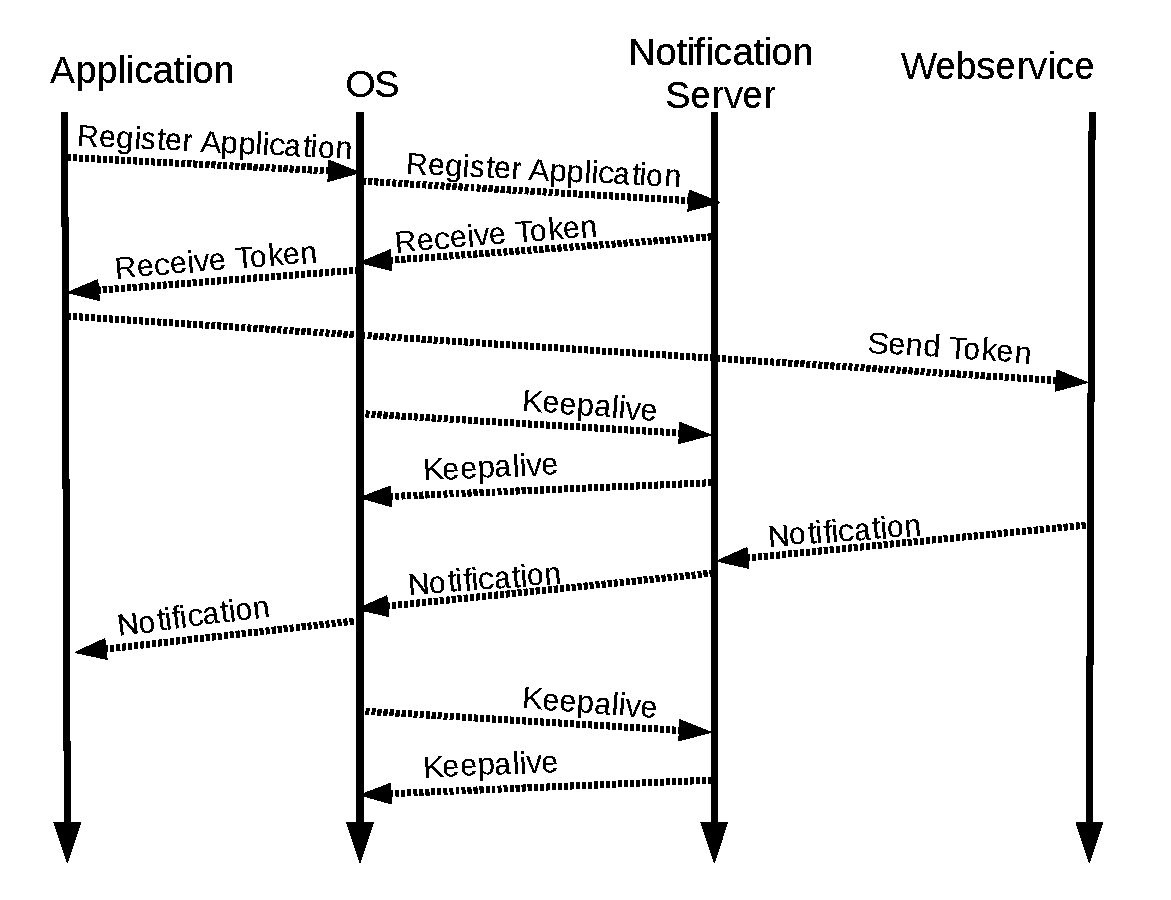
\includegraphics[width=\columnwidth]{figures/Notification.pdf}
\caption{Notifications on mobile OSes. \emph{Because notification messages are sent over TCP, keepalive messages are periodically exchanged to ensure TCP connections do not timeout.}}
\label{fig:push-expt-interarrival}
\end{figure}



\subsection{Controlled Experiment on Factory Reset Devices}

We first detail the detail the behavior of notification services by performing a controlled experiment on \emph{factory-reset} devices. 
The objective of this experiment was to analyze notification services for devices that are used \emph{out of the box}, and detail the impact of device manufacturer, and pre-installed applications. 

For our experiment, we performed a \emph{factory reset} on an iPod Touch, an iPad, an iPhone, a Samsung Galaxy SIII, and a Google Nexus S Phone; the reset was performed after their batteries were fully charged. 
We then perform the initialization step and assigned a dummy email account as the primary account to each of these devices.
We then allowed these devices to connect to the Internet over \wifi through \platname and monitored the Internet traffic from these devices.
We then studied the impact of access technology by letting the iPhone and Samsung Galaxy SIII tunnel traffic through \platname using cellular networks. 

We observed that the traffic volume during the 24 hour periods varied from 19~KB to 97~KB depending on the devices. 
We classify APNS and GCM messages using the TCP port numbers mentioned in their specifications~\cite{gcm, apns}.
Because we did not run any applications in the foreground, notification messages were responsible for largest fraction of the traffic volume; the share was 35\% for Nexus S, 88\% for the Samsung SIII and around 50\% for each of the iOS devices. 
The share of DNS traffic varied from 10\% to 40\% for each of the devices while the other services contributed to less than 10\% of the traffic volume.
The only exception was the Samsumg Galaxy SIII which used location services that contributed to 26\% of 47~KB traffic volume generated by the device.

\begin{figure}
\centering
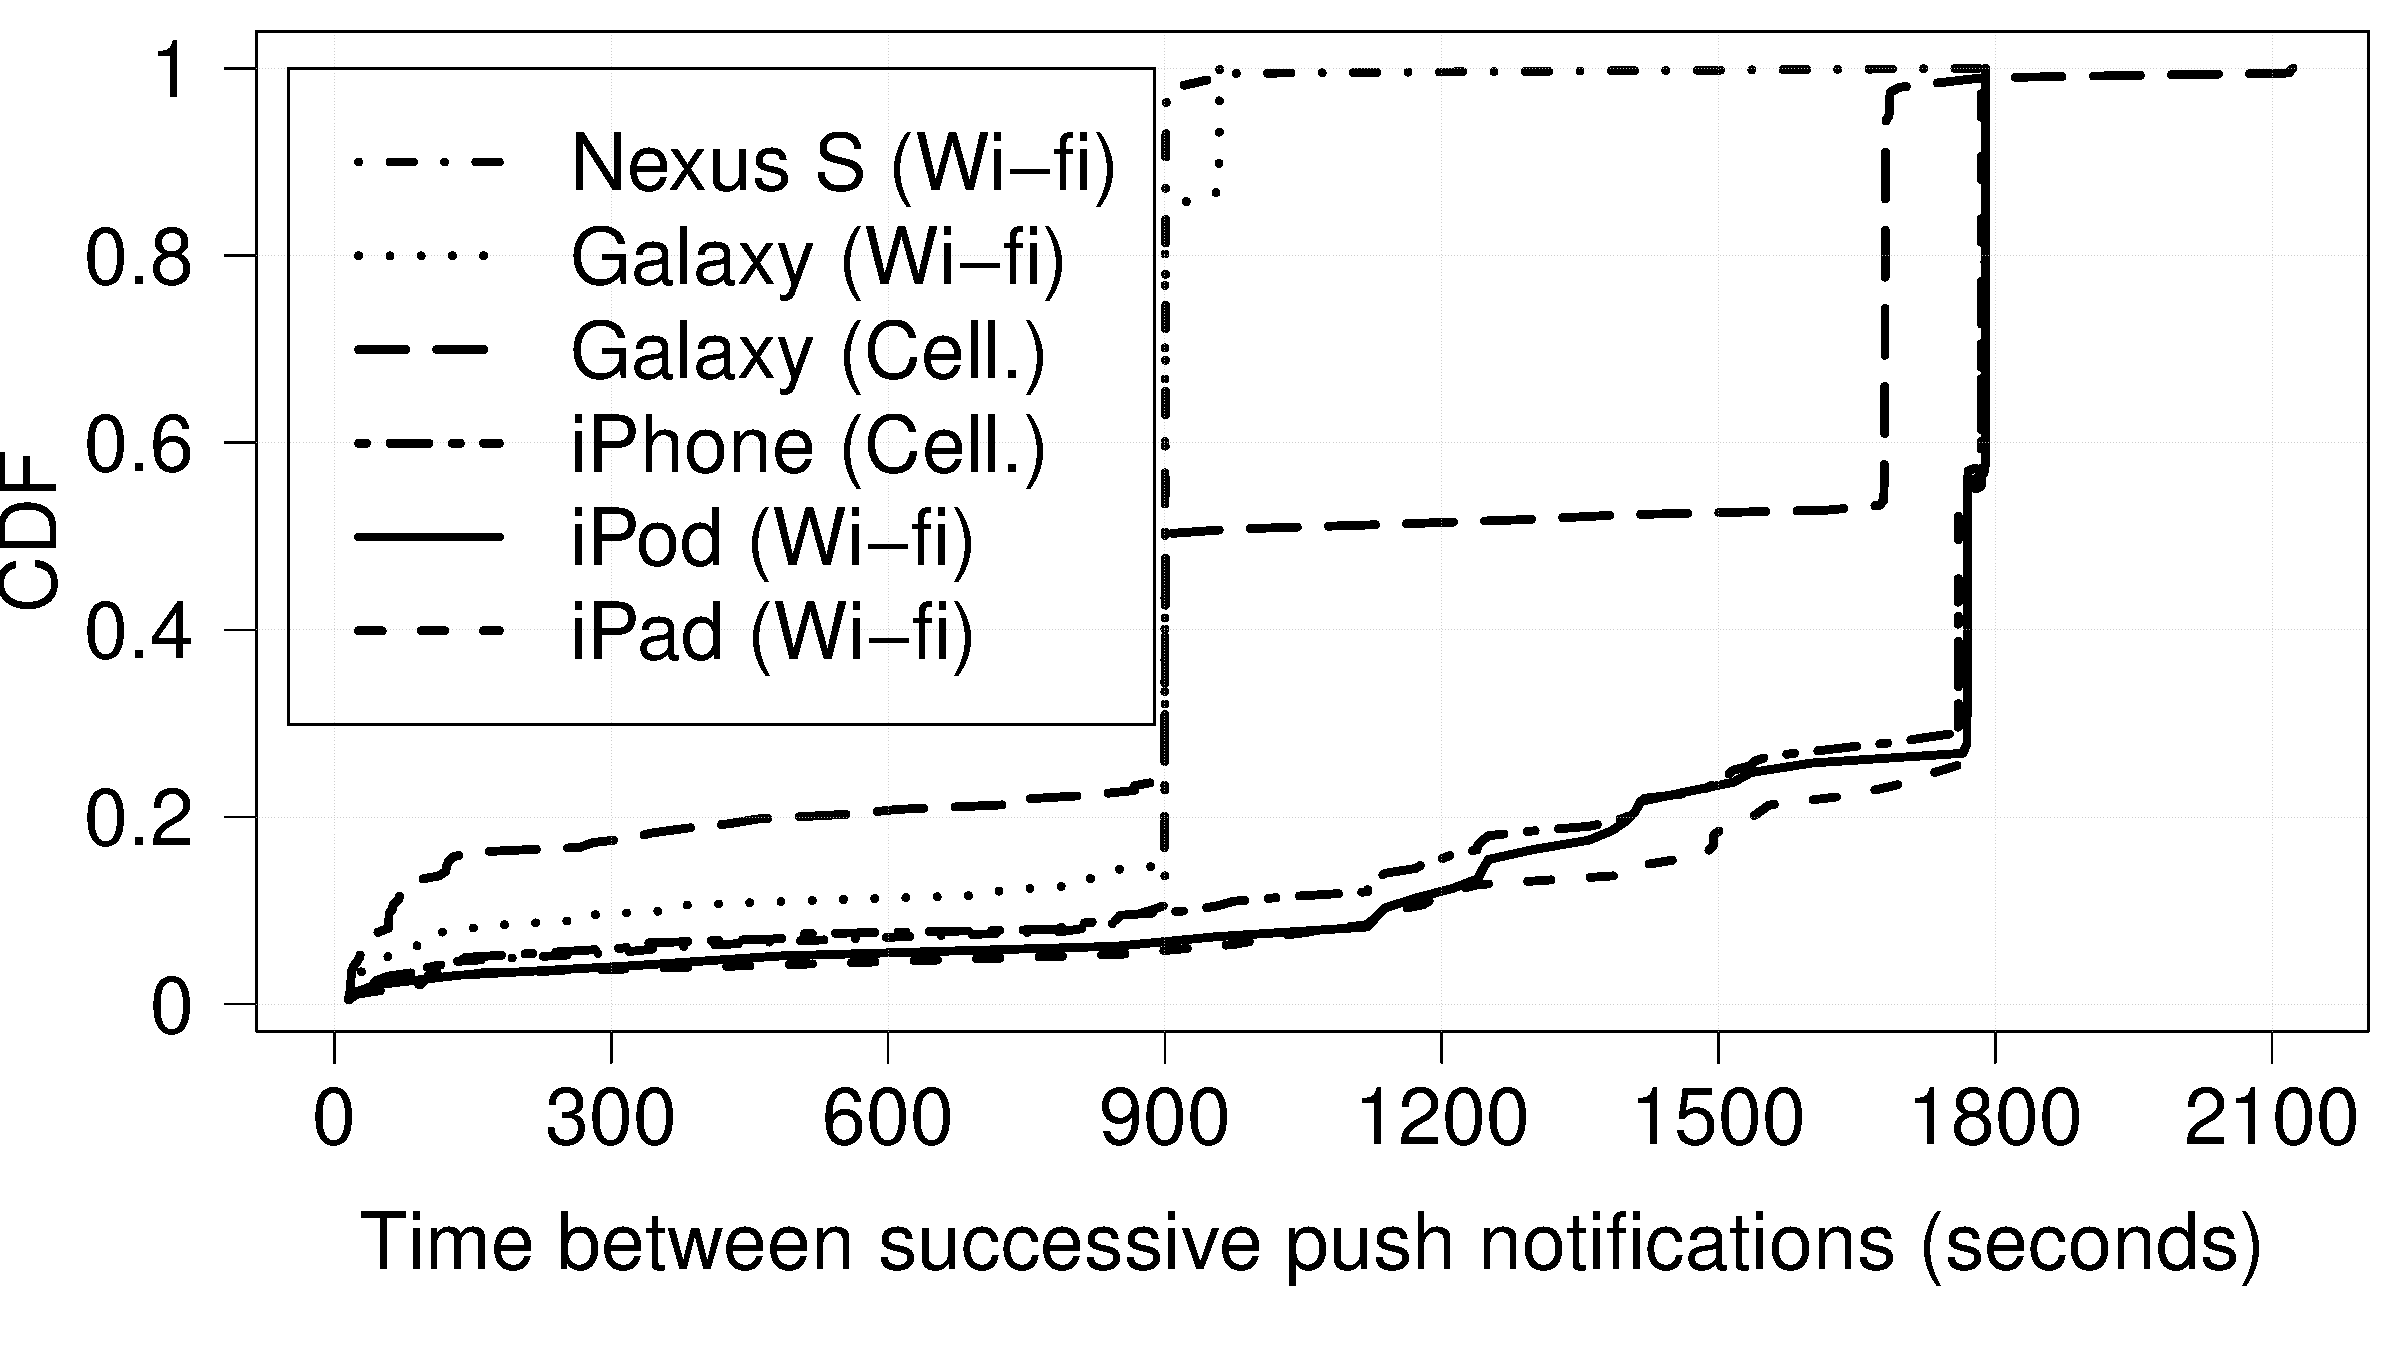
\includegraphics[width=\columnwidth]{plots/push_factoryreset_interarrival_distrib.pdf}
\caption{Inter-arrival time between notification messages after factory reset. \emph{The Android and iOS devices communicate with the notification server approximately once every 900~seconds and 1800 seconds respectively. The behavior of Android devices depends on the device, the pre-installed applications, and the access technology.}}
\label{fig:push-expt-interarrival}
\end{figure}

In \fref{fig:push-expt-interarrival} plot the time between successive messages sent by the notification servers on the ports assigned for notifications. 
We observe that the inter-arrival time between notifications for the Android devices is at least 900 seconds for more than 80\% of the notifications observed. 
The distribution of the inter-arrival time also depends on the access technology for the Samsung Galaxy SIII phone; we observe steps in the distribution for the SIII phone while we do not observe these steps when the same phone uses \wifi. 
We do not observe this difference when the Nexus S phone used the cellular data connection; we do not present the figure due to lack of space. 
\tbd{AR: Why these difference -- which applications stop coming up and so on}.
For the iOS devices, we observe an inter-arrival time at least 1700~seconds for that more than 75\% of the notifications in \fref{fig:push-expt-interarrival}. 
We do not observe a significant difference between the inter-arrival times for the iPhone over cell and \wifi and we do not present these results due to lack of space. 

On analyzing the packets exchanged, we observe that  all Android flows with an inter-arrival time larger than 800 seconds consisted of an empty TCP packet sent by the device followed by a 25 byte payload sent by the server.
Similarly, all iOS flows with an inter-arrival time larger than 1500 seconds began with an TCP packet with a payload of 85 bytes sent by the device followed by the server responding with of a TCP packet of 37 byte payload.

In summary, we observe notifications consume very little data, less than 50~KB in 24 hours, on Android and iOS devices in their default state.
The large time between successive notifications and the small amount of data exchanged implies they consume very little power.
We also observe that iOS devices have a larger time between successive notifications compared to Android devices in the default state. 
Furthermore, the inter-arrival time between notifications for Android devices differs based on the device manufacturer and the access technology. 

\subsection{Notifications In The Wild} 

We now characterize our observations on the notifications we observed in the \mobWild dataset. 
The objective of this analysis was to detail the frequency, traffic volume, and source of the notification services. 

\begin{figure}
\centering
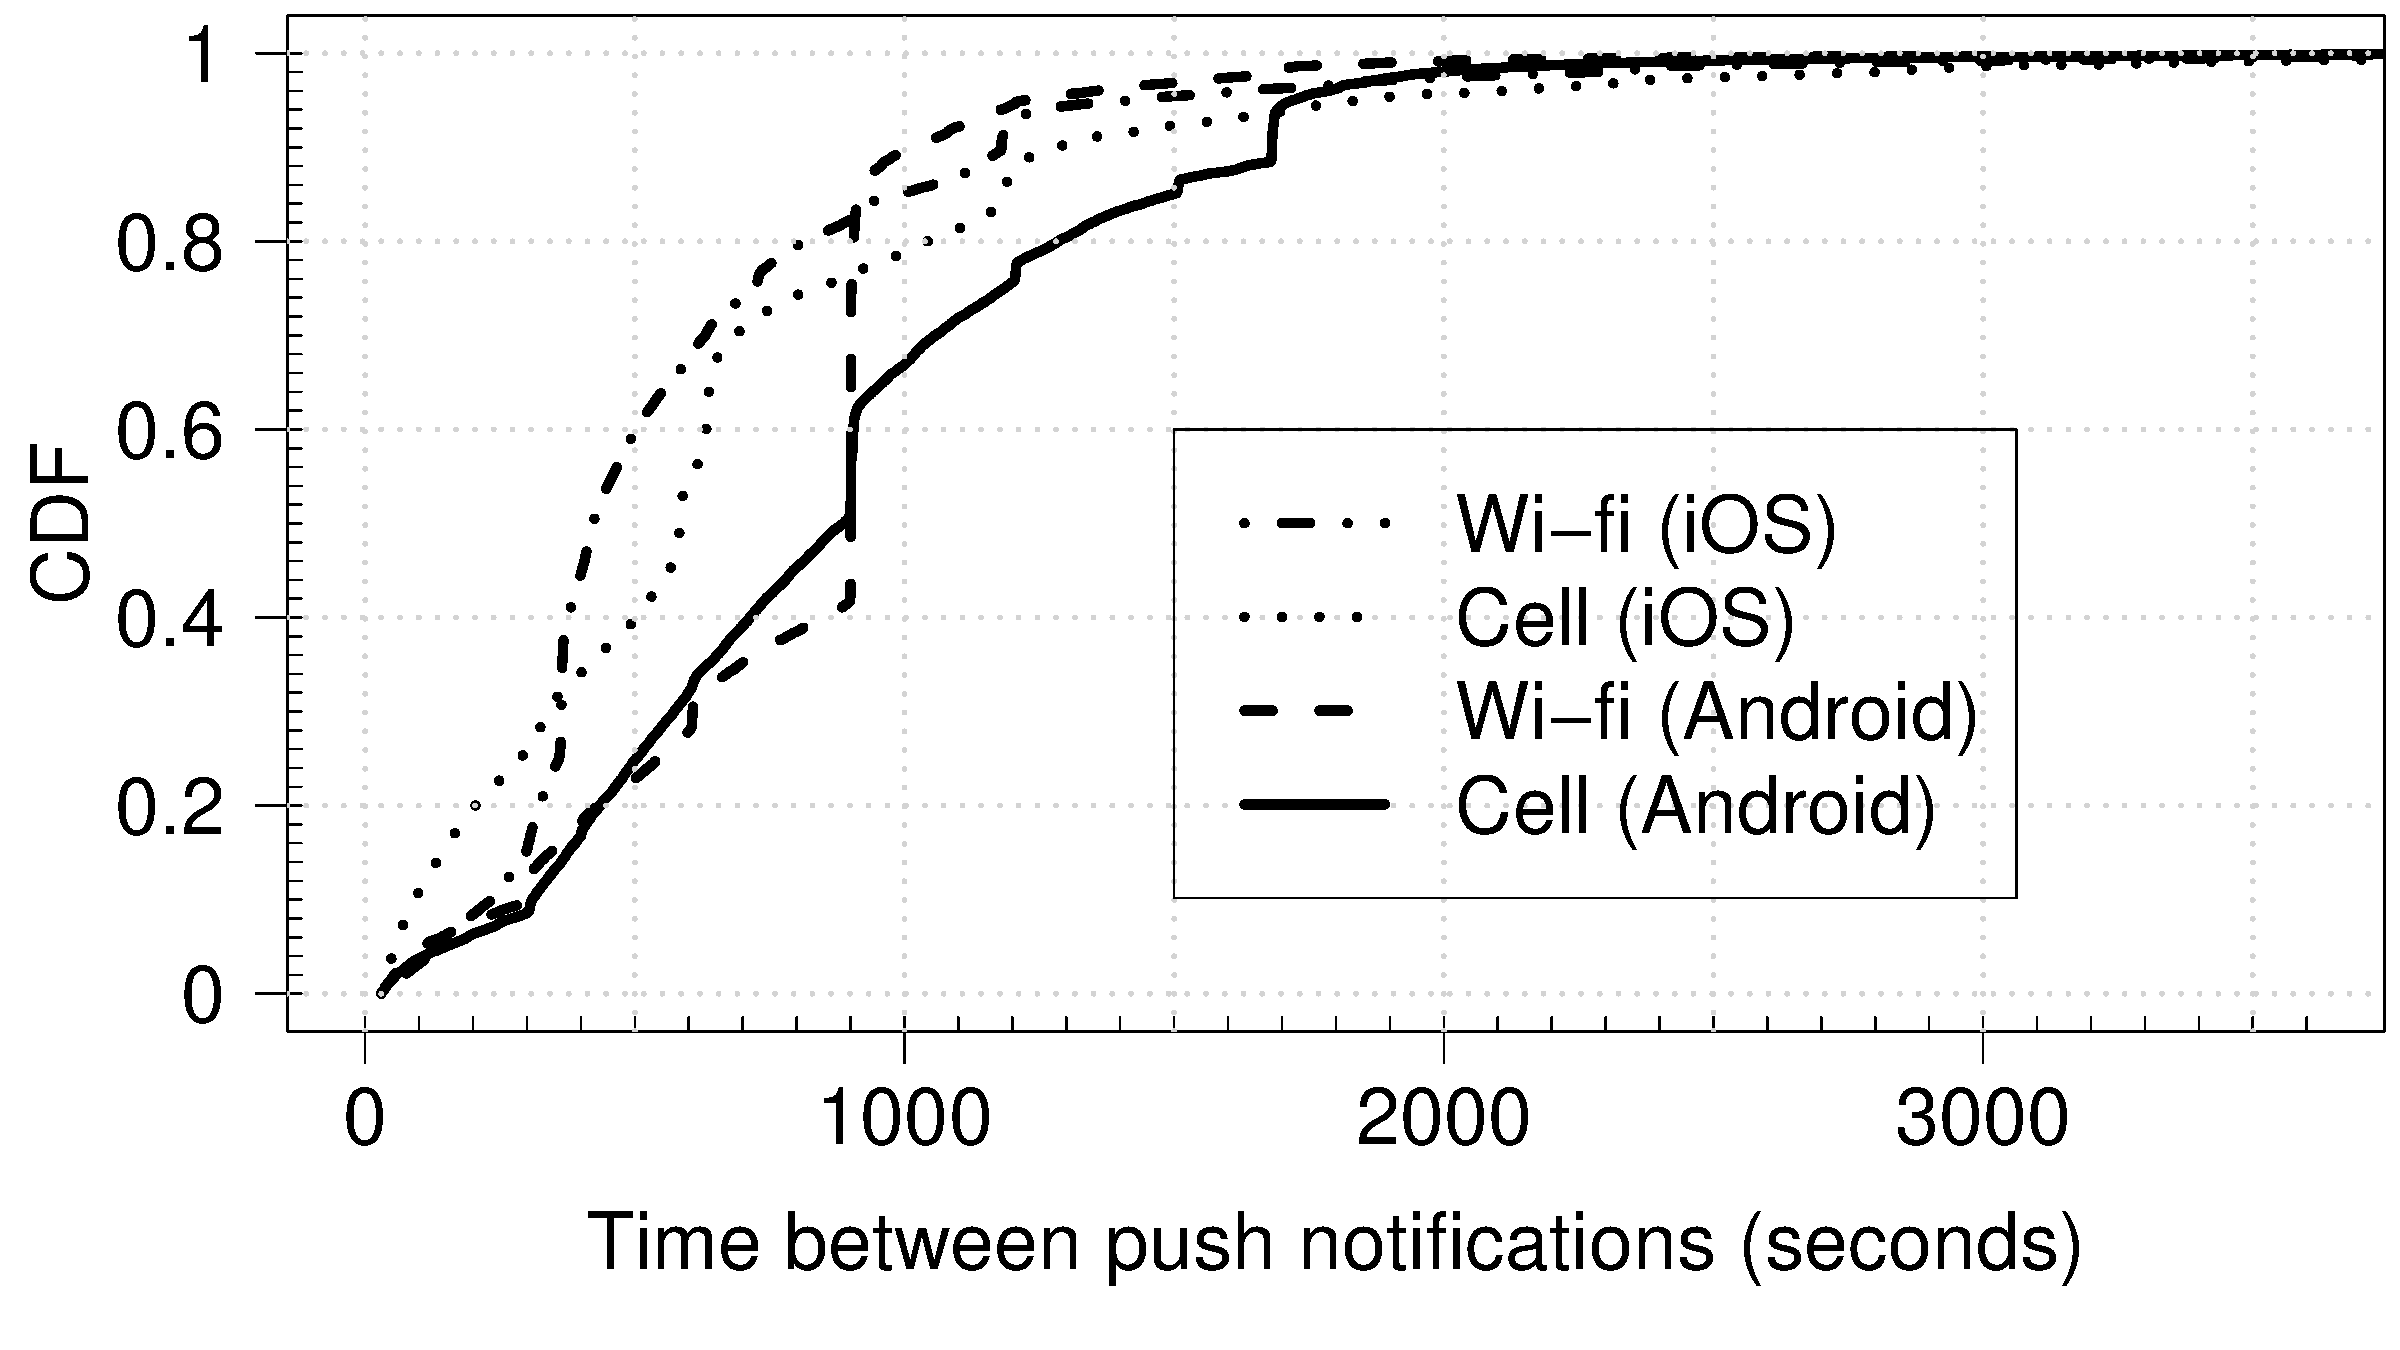
\includegraphics[width=\columnwidth]{plots/push_compare_os_tech_wild_distrib.pdf}
\caption{Distribution of the time between push notification messages in the wild. \emph{The frequency of push notification messages is higher for the iOS devices in our dataset compared to the Android devices. Notification messages are less frequent over cellular networks compared to Wi-Fi networks.}}
\label{fig:push-wild-compare-ostech}
\end{figure}

%The advantage of \platname is that it allows for direct comparison between devices across and their behavior across access technologies. 
To analyze the frequency of notification messages, we plot the distribution of the time between successive push notification messages for Android and iOS devices over cellular and \wifi networks in \fref{fig:push-wild-compare-ostech}.
In \fref{fig:push-wild-compare-ostech} we observe that a higher time between push notifications over cellular networks in comparison to \wifi networks for iOS and Android devices.  
We also observe the Android devices in our dataset receive notifications less frequently compared to the iOS devices in our dataset. 
We also observe a heavy tail for the time between notification messages which implies potentially long idle intervals.
\tbd{Correlation between time between notification messages and size of the next idle time observed?}


\begin{figure}
\centering
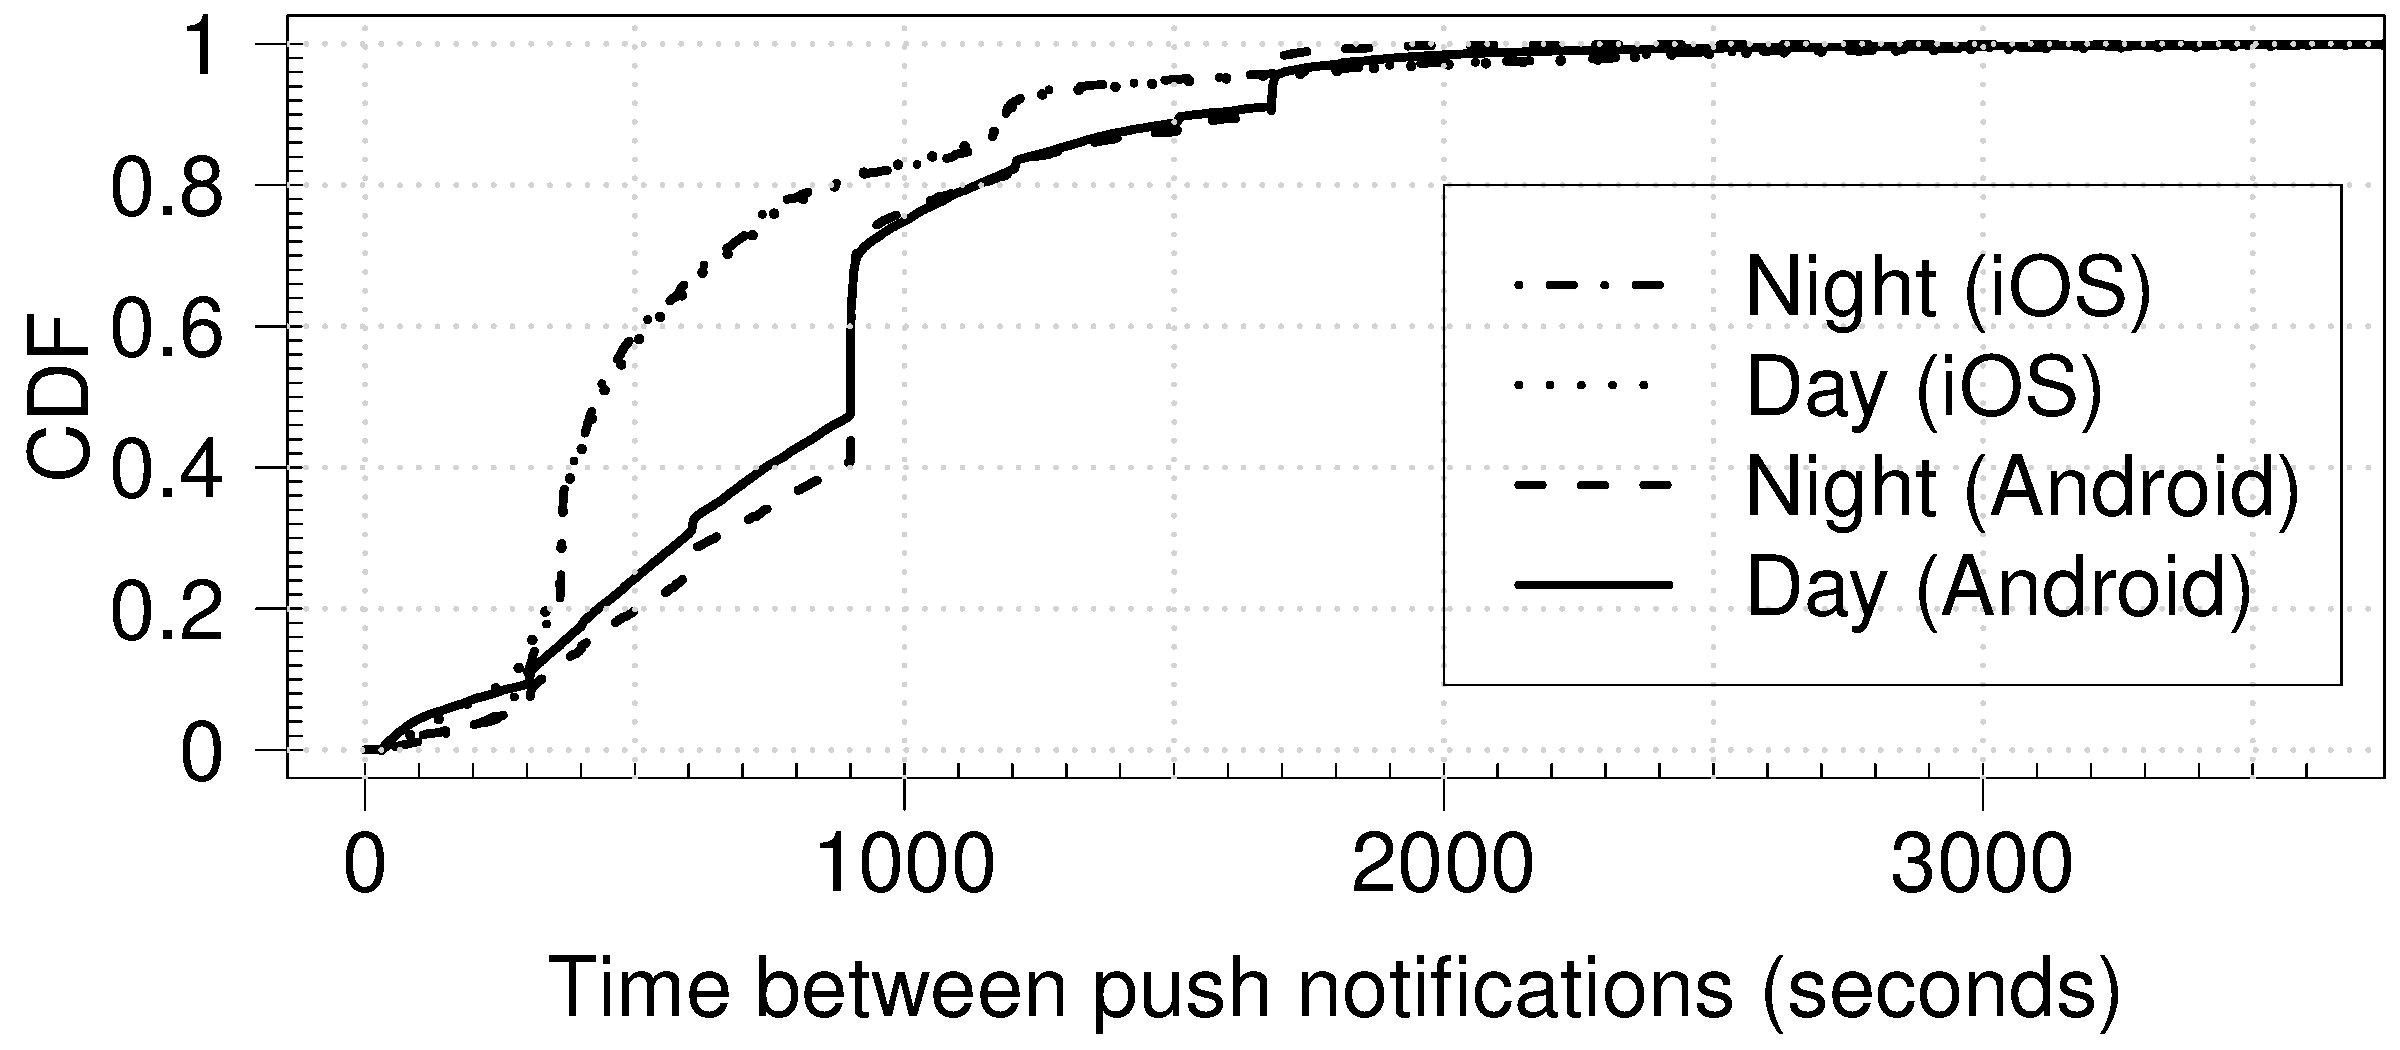
\includegraphics[width=\columnwidth]{plots/push_compare_diurnal_wild_distrib.pdf}
\caption{Impact of time-of-day on the push notifications. \emph{The rate of notifications is agnostic of the time of the day for iOS and Android devices.}}
\label{fig:push-wild-diurnal}
\end{figure}

The notification messages could be in response to user actions, for example, a mail server might receive a notification of a new message.
To analyze this impact, we notification messages received during two time intervals: from midnight to 6 am (night), and from 6 am to midnight (day). 
In \fref{fig:push-wild-diurnal}, we plot the distribution between successive notification messages for these two intervals. 
We observe that the Android and iOS devices appear to be agnostic of the time of the day. 
The iOS devices (from verion 6.0) come with a feature called \emph{Do Not Disturb (DND)} that does raise notification alarms on receiving notifications during specific time periods. 
We observe notification messages were received by the device that had enabled this feature during the intervals their users had configured as \emph{Do Not Disturb}.

\begin{figure}
\centering
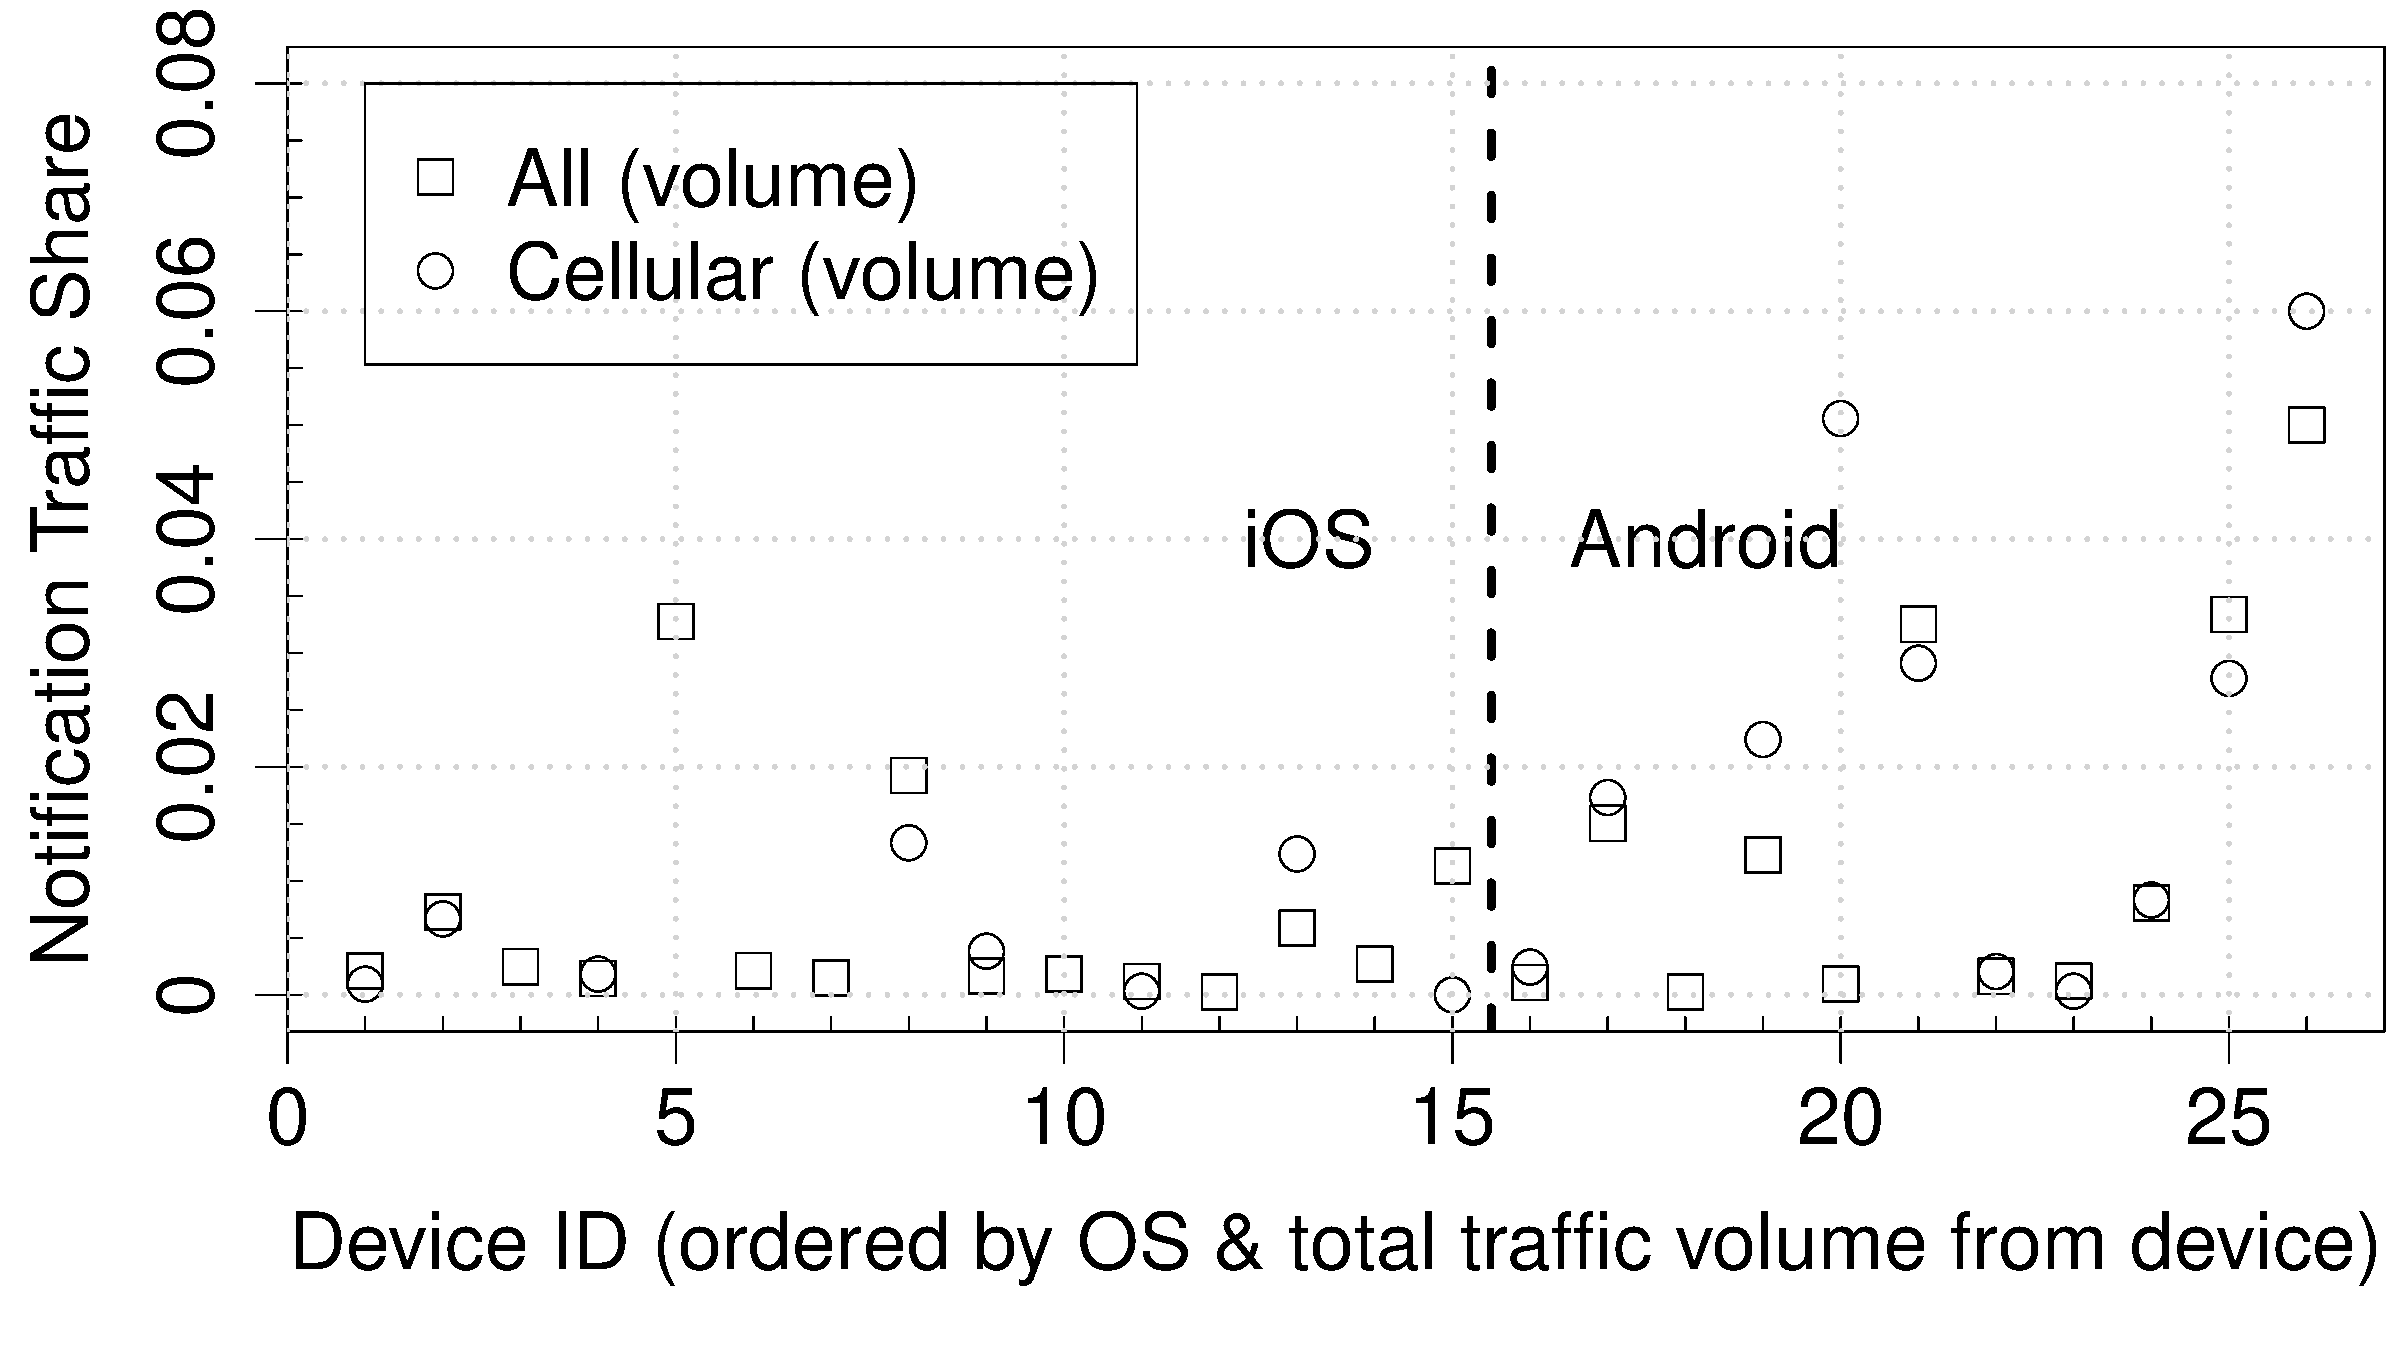
\includegraphics[width=\columnwidth]{plots/push_compare_trafficshare.pdf}
\caption{Traffic share of push notifications. \emph{Push notifications are responsible for less than 5\% of the traffic volume on most devices.}}
\label{fig:push-traffic-share}
\end{figure}

To analyze the volume of notification messages, we plot the share of notification messages as a fraction of total traffic from the device in \fref{fig:push-traffic-share}.
We observe that the notification messages are responsible for less than 4\% of the traffic volume on most Android and iOS devices. 
In \fref{fig:push-traffic-share}, we also plot the share of notification messages when the device exchanged data over cellular networks. 
We observe that there is no significant difference in the traffic share of notification messages when the device used cellular traffic. 
\tbd{Why do we care?}

To further analyze the source of the notification messages we analyzed the DNS lookups that were performed before the connections for receiving notification messages was established. 
We observed that the servers that pushed content to iOS devices correspond to the DNS requests that match the pattern \emph{*courier.push.apple.com} and \\ \emph{*courier-push-apple.com.akadns.net}.
For the android devices we observe that the DNS requests match the pattern\\ \emph{*talk.google.com}. 

In summary, we detail the behavior of the notification services using controlled experiments and the \mobWild dataset.  
We observe that push notifications consume a small fraction of the data and exhibit a heavy tail for the time between successive messages. 
We also observe that the frequency of notification messages was agnostic of the time of the day. 
Furthermore, notification messages were received by iOS devices even during the time interval the users had configured \emph{Do Not Disturb.}


% \begin{packedenumerate}
% \item How frequently do Push notifications take place in the wild?
% \item What is the impact of access technology on push notifications?
% \item What is the impact of the time of the day?
% \item What is the volume of push notification traffic?
% \item From which hosts are these notifications received?
% \end{packedenumerate}

%\subsection{Discussion}




% OLD TABLE WITHOUT IPHONE
% \begin{table}
% \begin{small}
% \begin{tabular}{|c|c|c|c|c|}
% \hline
% \multirow{2}{*}{\bf Application} & \multicolumn{4}{c|}{\bf Traffic Share in the first 24 hours}\tabularnewline
% \cline{2-5}
%      & iPad & iPod & Galaxy SIII & Nexus \tabularnewline
%      & (19 KB) & (21 KB) & (47 KB)& (97 KB)  \tabularnewline
% \hline
% Notifications & 0.54 & 0.53 & 0.35 & 0.88 \tabularnewline
% \hline
% Location & 0 & 0 & 0.26 & 0 \tabularnewline
% \hline
% SSL & 0 & 0 & 0.30 & 0.11 \tabularnewline
% \hline
% Mail & 0.05 & 0.07 & 0 & 0 \tabularnewline
% \hline
% HTTP & 0.13 & 0 & 0.09  & 0 \tabularnewline
% \hline
% UDP & 0.28 & 0.40 & 0.01 & 0.01 \tabularnewline
% \hline
% {\em total}& {\em 1.0} & {\em 1.0} & {\em 1.0} & {\em 1.0}\tabularnewline
% \hline
% \end{tabular}
% \end{small}
% \caption{Network usage in the first 24 hours after factory reset. \emph{Notifications contribute to the largest fraction of traffic volume across all devices.}}
% \label{tab:traffic-share-factory-reset}
% \end{table}

%While computing this distribution, we account the diversity in device usage in the following manner.
%For each device and each access technology we compute the 100 quantiles from 0.01 to 1.0 in steps of 0.01 of the time between successive push notifications. 
%We then use the median value of each quantile (from 0.01 to 1.0 in steps of 0.01) for a given access technology and operating system of the device.

% In \fref{fig:wild-inter-arrival-push} we present the time between successive push notifications for the 25 devices in our dataset. 
% As observed in \fref{fig:wild-cdf-push} we observe that the iOS devices receive push messages more frequently that the Android devices. 
% We also observe that the time between push notifications is higher for Android devices.
% The iOS devices prefer a cellular data connection for Push notification over \wifi \tbd{http://support.apple.com/kb/TS4264}. 
% However, in \fref{fig:wild-cdf-push} and \fref{fig:wild-cdf-push} despite this preference, we observe that the time between successive push notifications for iOS devices is higher over cellular networks in comparison to \wifi networks.  
% We observe that \tbd{SSL traffic} to mail servers was followed \tbd{x\%} after push notifications.
% This implies that higher usage of the device over \wifi may result in a higher number of notificatons received. 
% In \fref{fig:wild-inter-arrival-push}, device ID 
%Only if the cellular connection is not available or viable will the device switch to Wi-Fi for APNs connections.


\section{Application Characterization}
\label{sec:characterize-app}

  We now turn to measurements of specific popular iOS and Android applications. 
  When users install apps, they grant them Internet access without detailed knowledge of how that access will be used, including {\it how much} data is sent or accessed, {\it what} data is sent,  or {\it with whom} the app communications.
  ``How much'' is important to conserve both bandwidth caps and battery capacity: an app which consumes or produces too much data will waste bandwidth resources, while an app which consumes or produces data too frequently will prevent the device radio from going idle to save power.
  ``With whom'' is important to protect users from excessive tracking -- the more organization's servers an app connects to, the more organizations which are able to track user behavior, location, or other private data.
  Finally, ``what data'' is important because apps may unnecessarily leak personally identifiable information (PII) such as user email address, IMEI, contact information, or other stored data either to the app provider or worse, to any eavesdropper on a public WiFi connection.
  We  report on our findings in all three of these dimensions for the iPhone and Android apps in our study.

\subsection{Bandwidth and Radio Usage}

  {\bf In the Wild.}
    \begin{itemize}
      \item Stats on how much bandwidth each user used; time of day; how frequent...
    \end{itemize}

  {\bf Android Apps.}
    To dig in to the root cause of these usage patterns, we also did an `app-by-app` analysis of network usage to see if most bandwidth consumption/radio time was the result of a few heavy applications, with most applications relatively idle, or whether usage was divided amongst all applications equally.
    In Figure~\ref{fig:app-by-app-usage}, we plot the CDF of total bytes transferred by each app in our study, one line for the top-100 Google Play apps we tested manually, and another for the top 2000 apps, tested automatically, from a third-party market.
    We see that...\tbd{Amy...}
    Regarding radio usage,...\tbd{Do we even have time to do this? I don't remember the exact metrics we used for the MobiSys submission.}

  {\bf iPhone Apps.}

\subsection{Third Party Servers}
  Many free applications support themselves financially by serving ads or providing resources for third parties to track user behavior.
  We now explore how many servers are contacted by a given app (\ie{} how many providers are tracking a user with this app) -- most of these typically for ads, tracking, or analytics -- as well as how much data is transferred to and from these servers (\ie{} how much does this traffic impact the user's data cap?).

  {\bf In the Wild.}
  We first consider the overall impact of these ads, analytic, and tracking services on typical user behavior in our IRB study...
  \tbd{Ashwin...}

\begin{figure}[t]
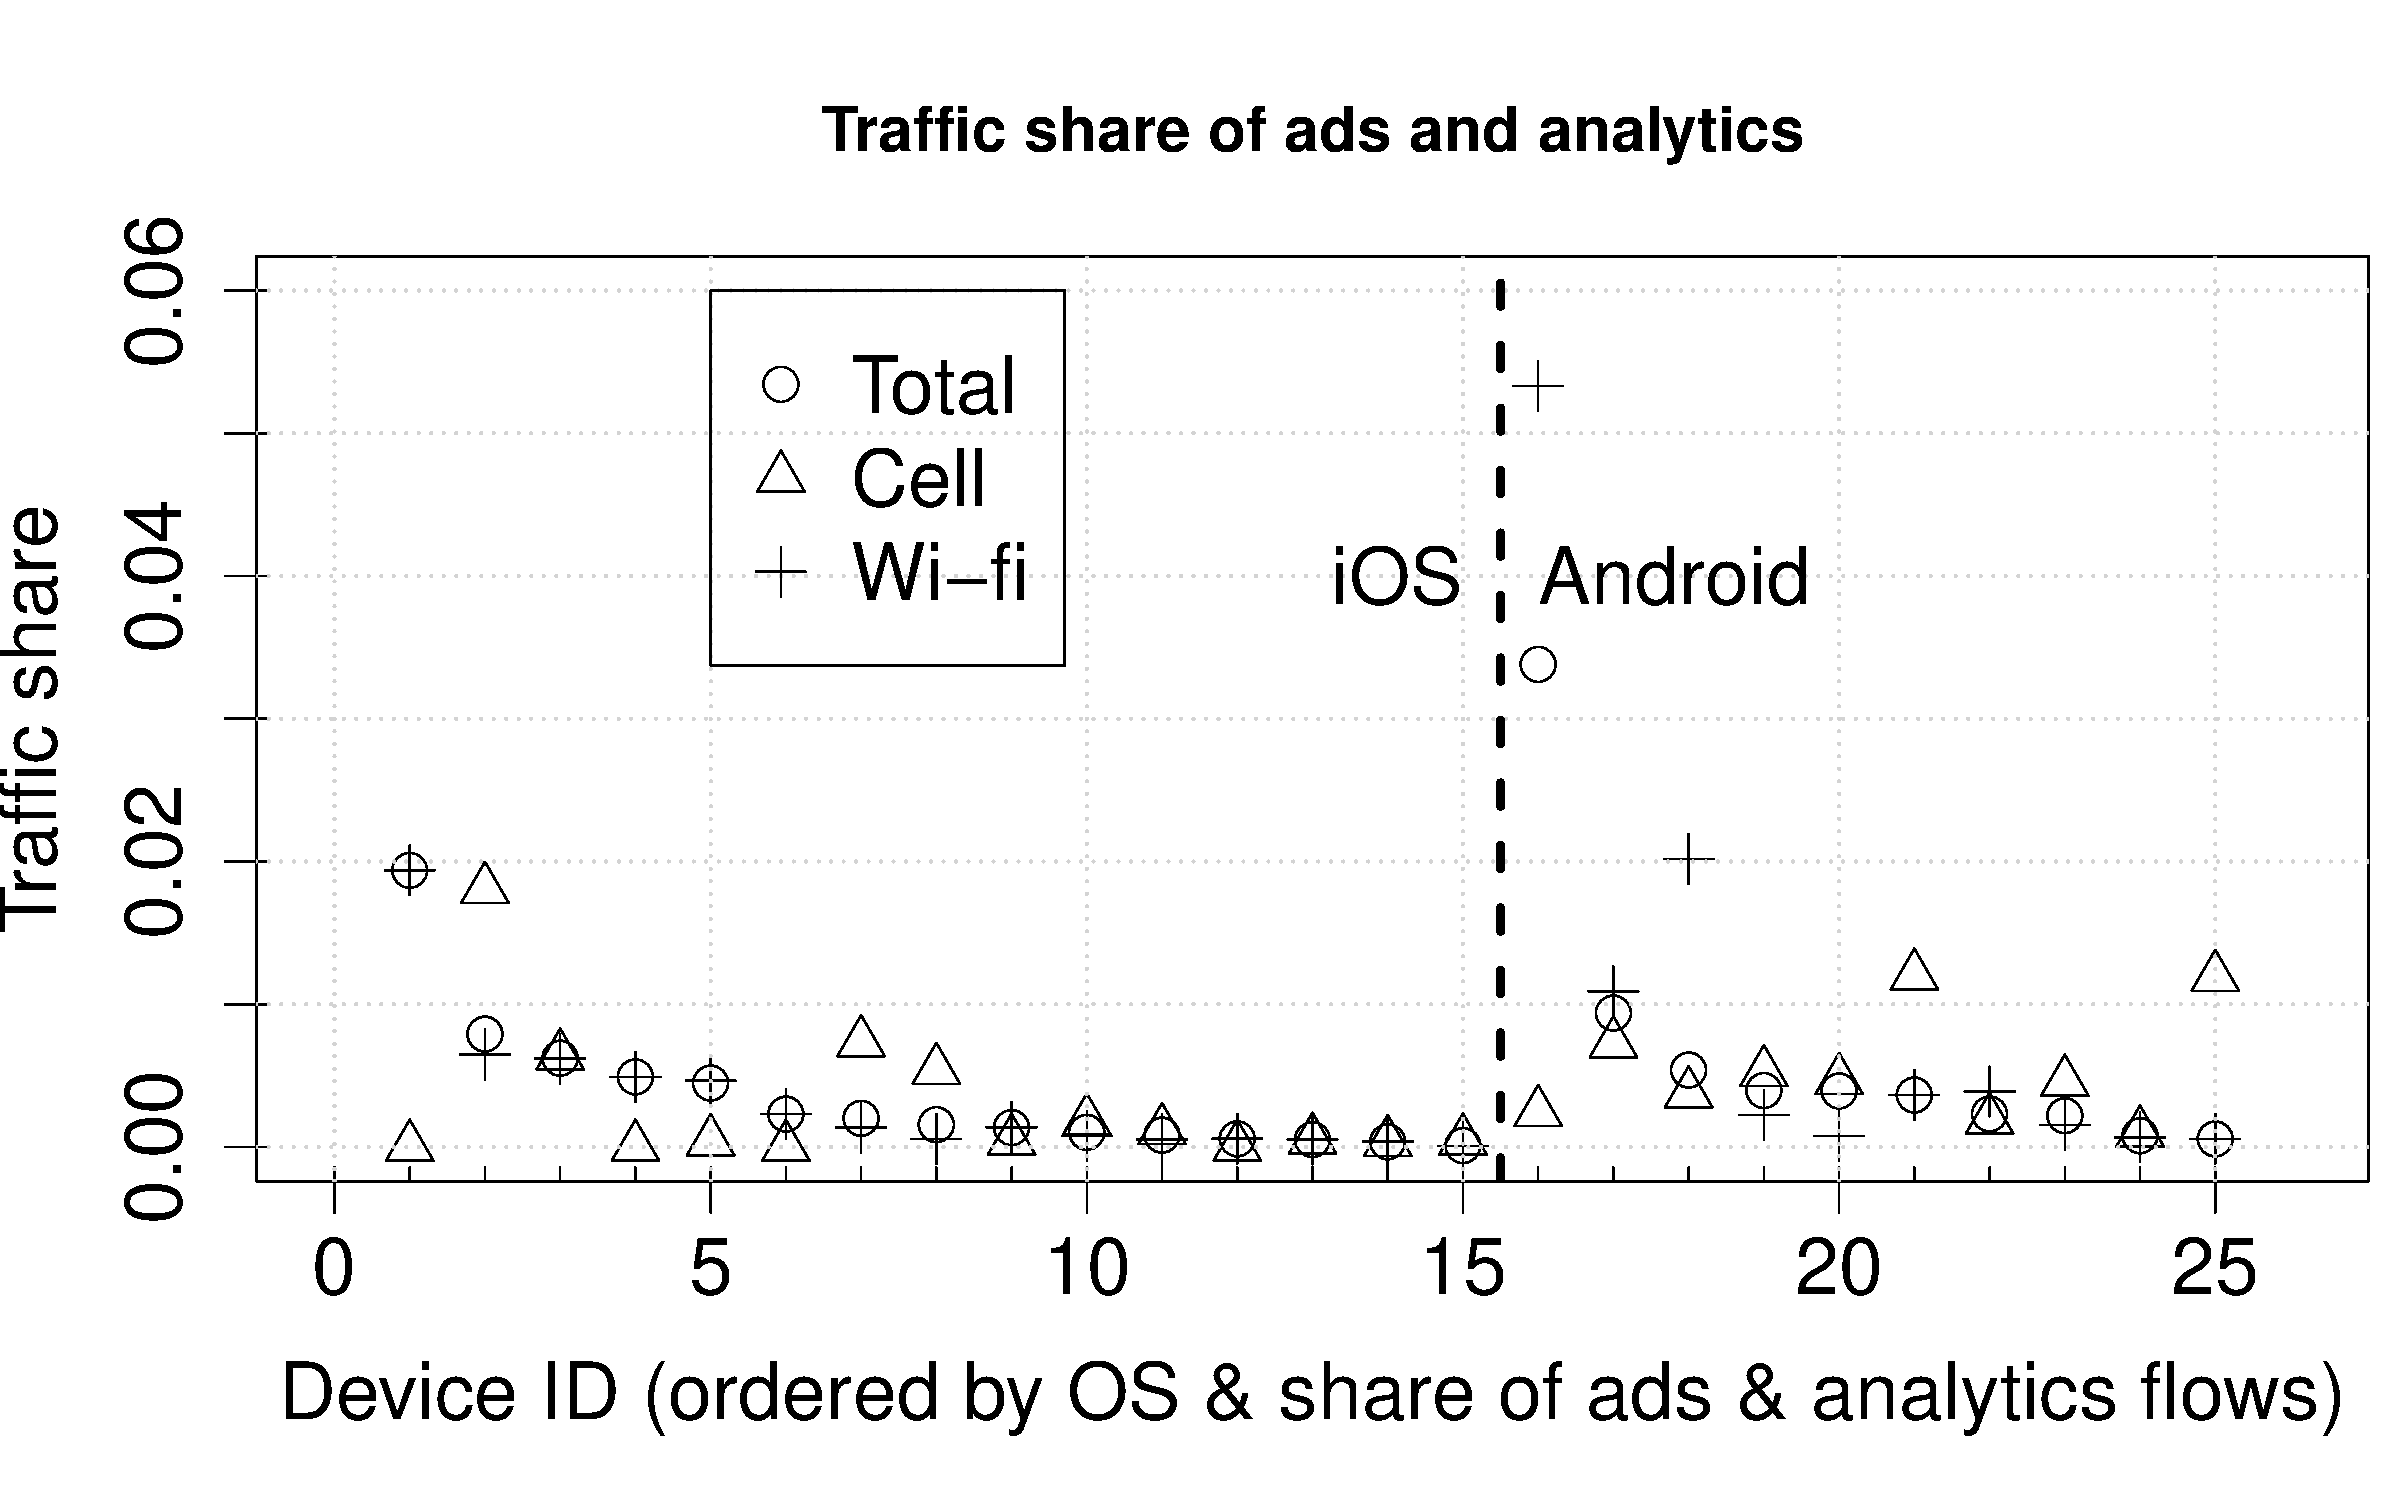
\includegraphics[width=\columnwidth]{plots/ad_share_bytes.pdf}
\caption{Fraction of traffic volume because of Ads and Analytics. \emph{\tbd{Check for id1 and id25}}}
\label{fig:description}
\end{figure}

\begin{figure}[t]
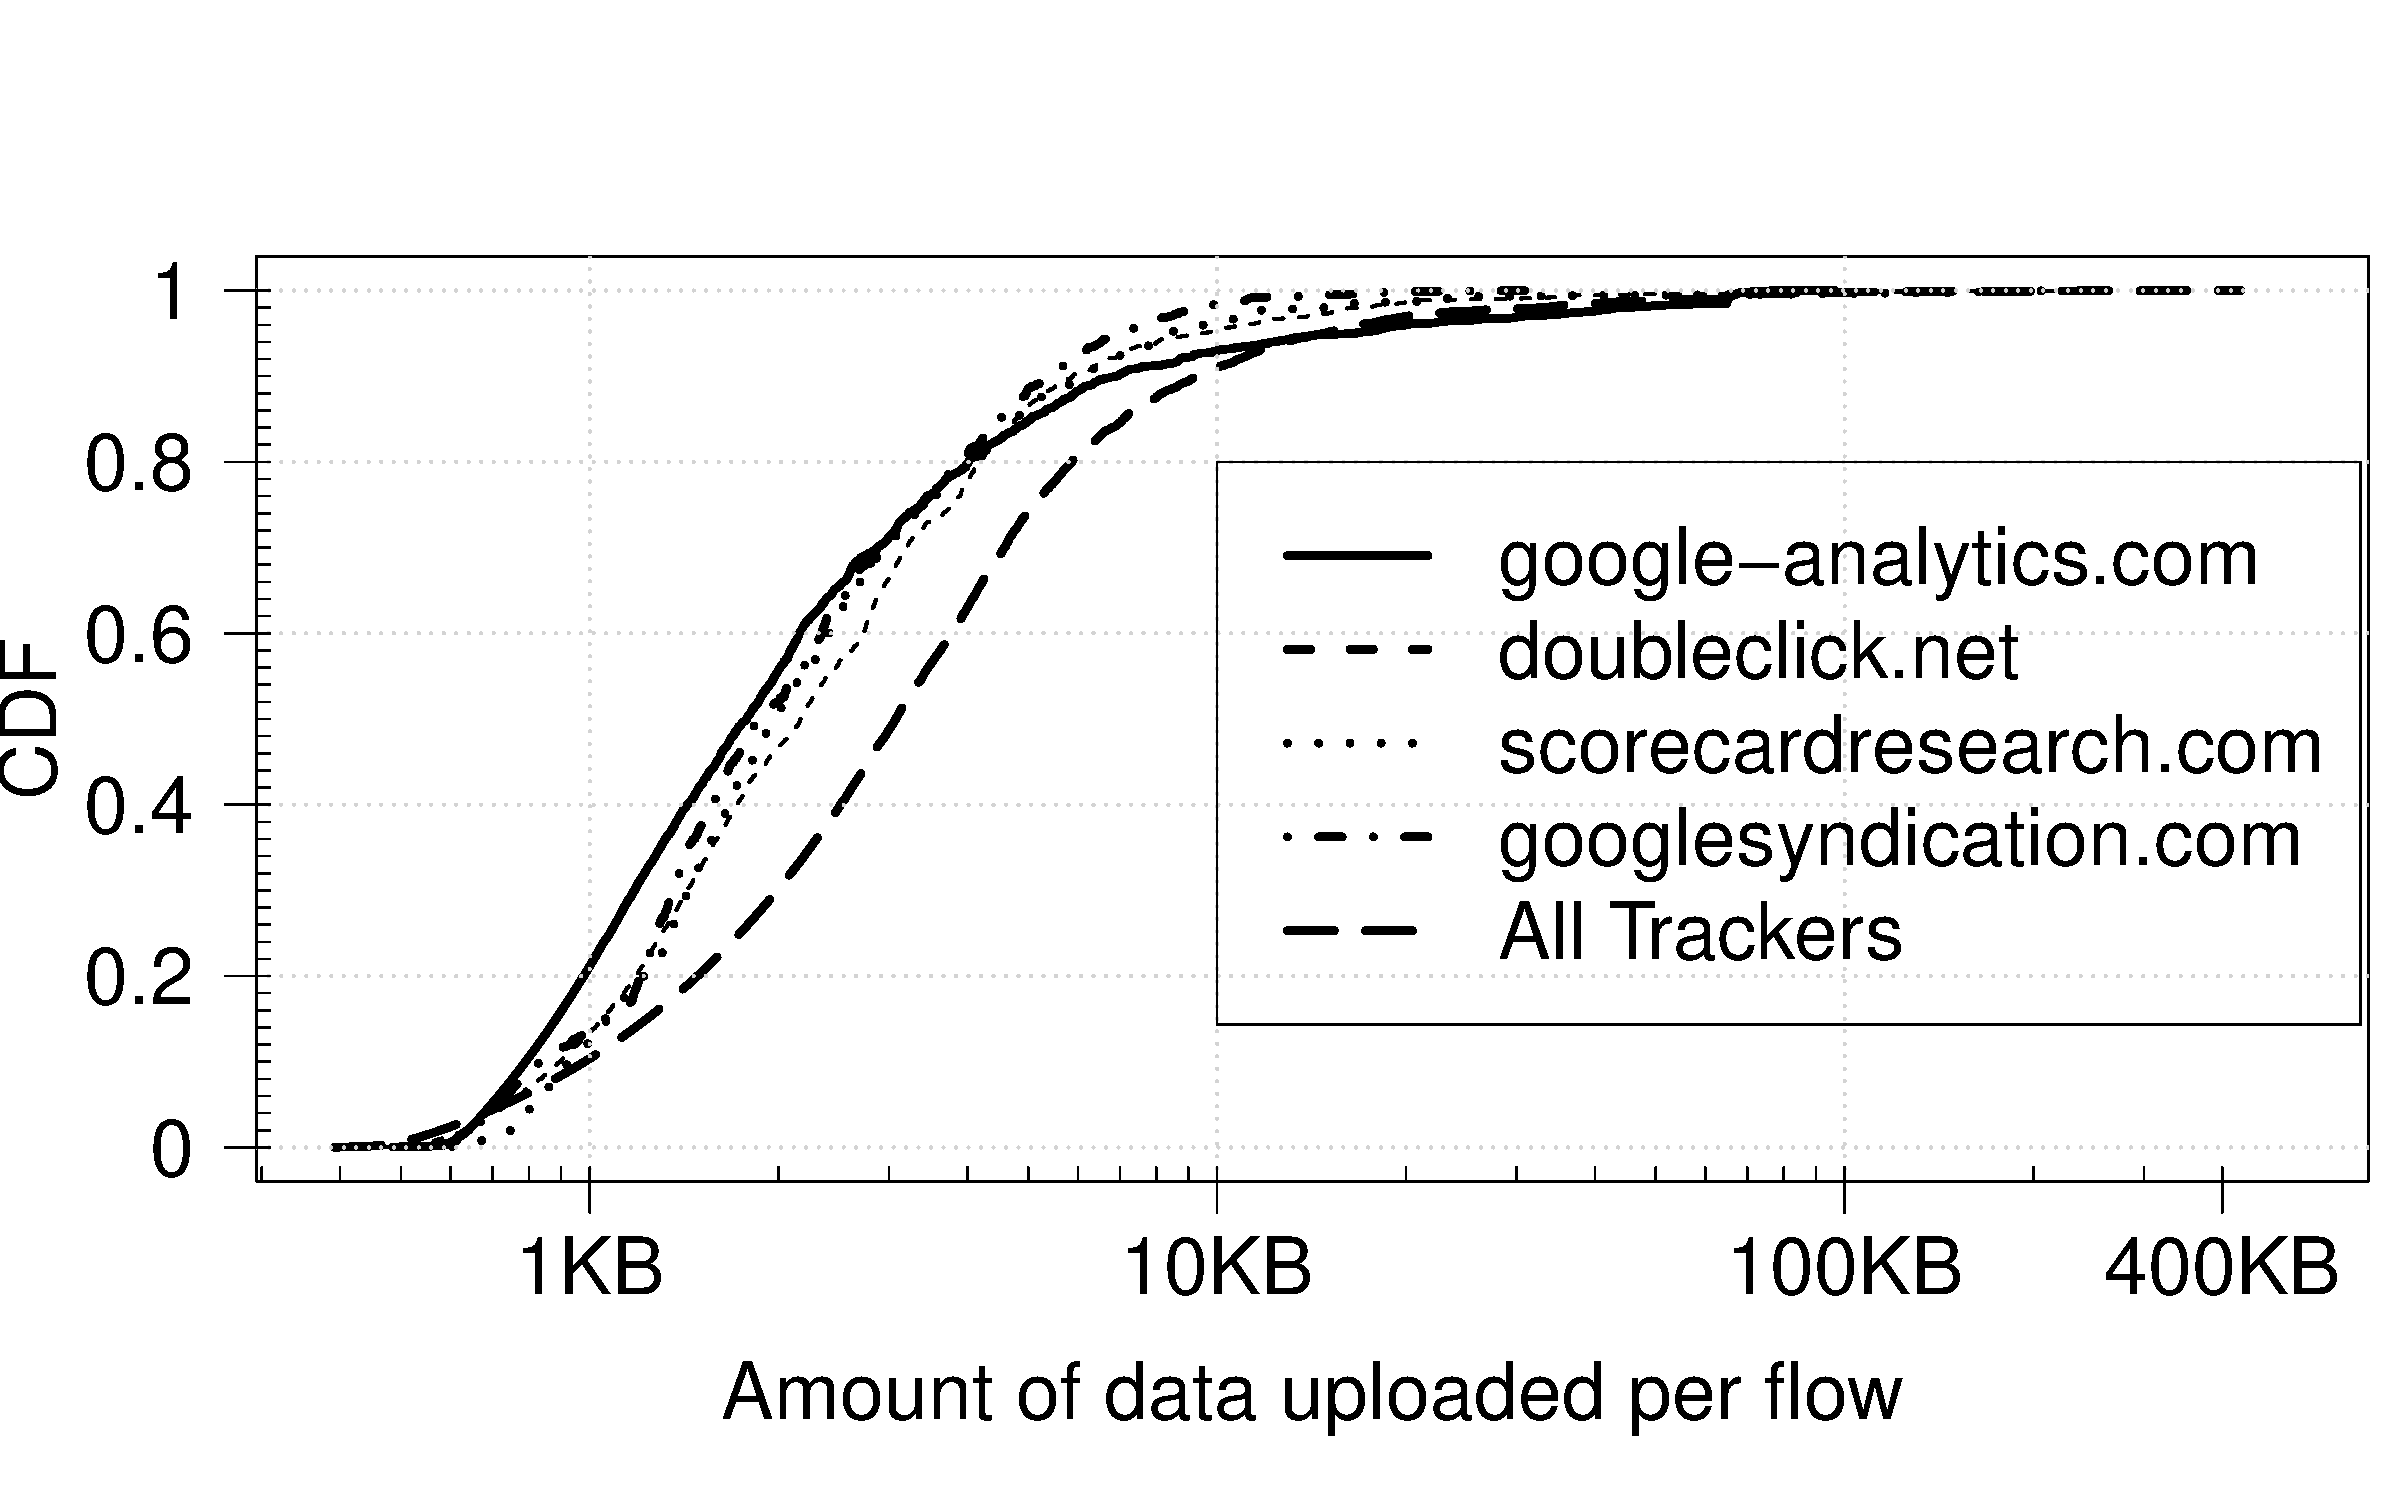
\includegraphics[width=\columnwidth]{plots/distrib_ad_uploads.pdf}
\caption{Distribution of bytes uploaded by ads and analytics sites. \emph{The distribution of bytes uploaded by all ads and analytics sites and the top four ads sites based on traffic volume across all users}.}
\label{fig:description}
\end{figure}

\begin{figure}[t]
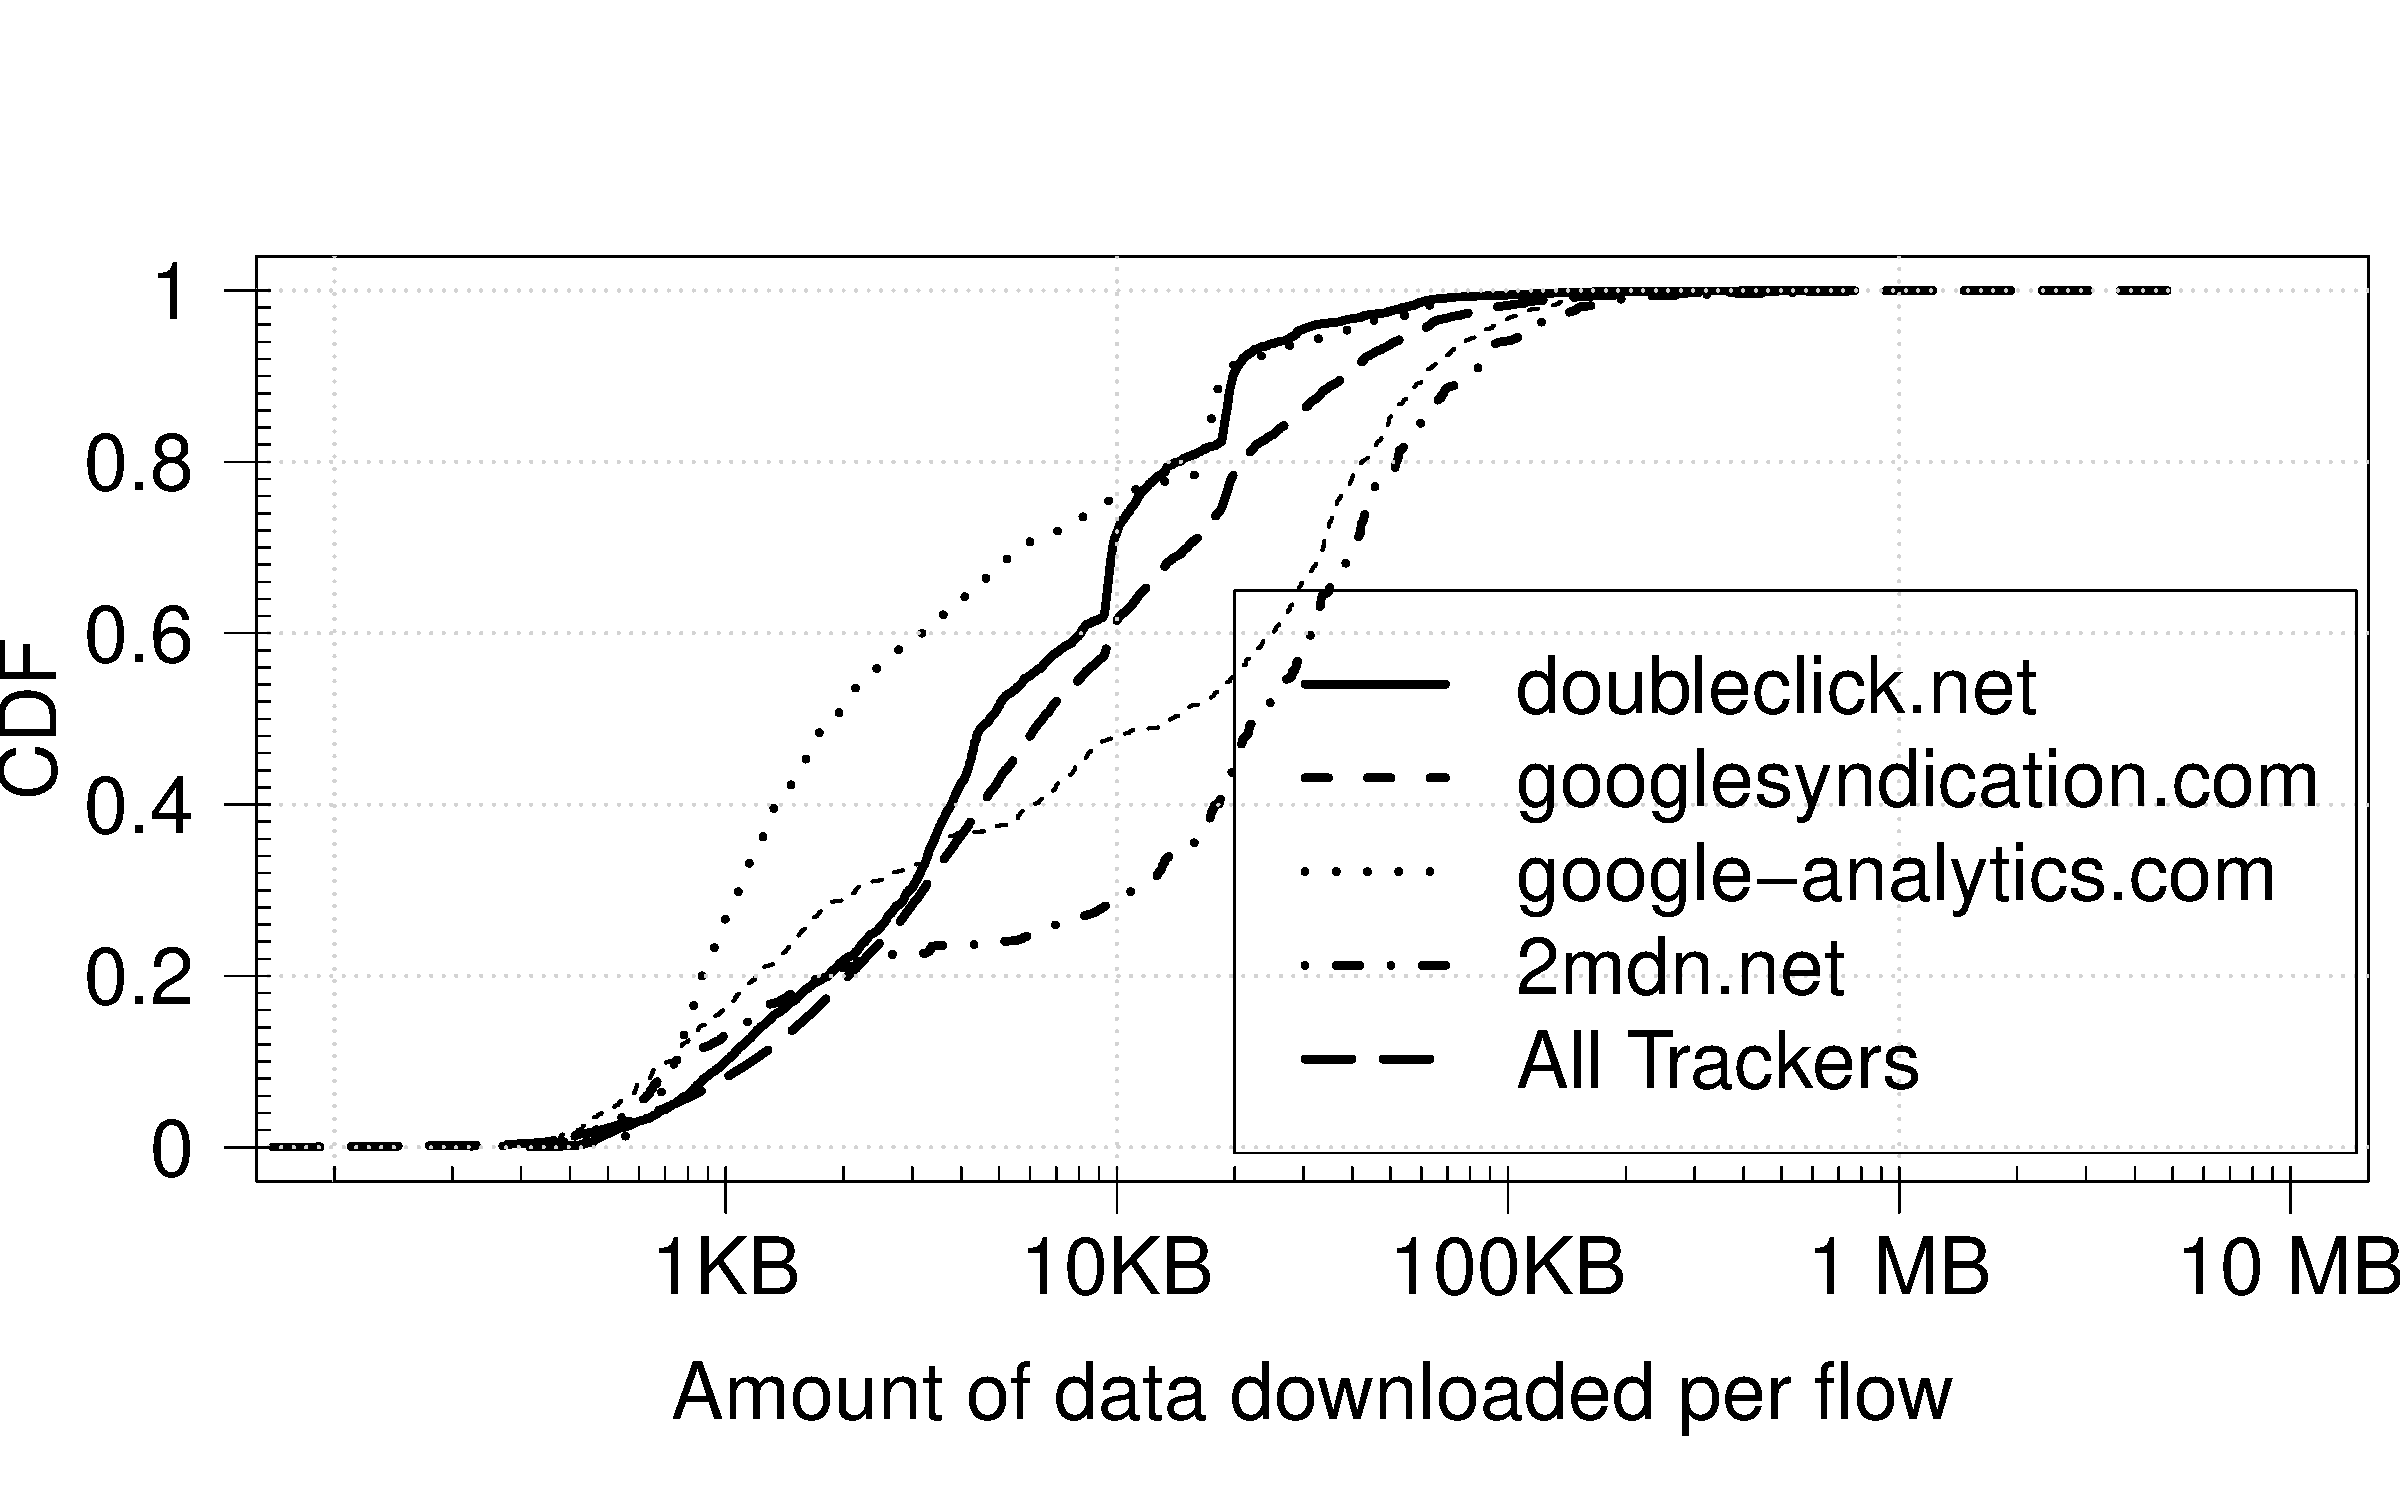
\includegraphics[width=\columnwidth]{plots/distrib_ad_downloads.pdf}
\caption{Distribution of bytes downloaded by ads and analytics sites. \emph{The distribution of bytes uploaded by all ads and analytics sites and the top four ads sites based on traffic volume across all users}.}
\label{fig:description}
\end{figure}

\begin{table}[t]
\centering
\begin{small}
\begin{tabular}{|p{0.35\columnwidth}|p{0.1\columnwidth}|p{0.15\columnwidth}|p{0.1\columnwidth}|}
\hline
\multirow{2}{*}{\bf Tracker} & \multicolumn{3}{c|}{\bf Number of devices tracked}\tabularnewline
\cline{2-4}
   &  {\bf Total} & {\bf Android} & {\bf iOS} \tabularnewline
\hline
doubleclick.net & 25 & 11 & 14 \tabularnewline
\hline
google-analytics.com   & 25 & 11 & 14 \tabularnewline
\hline
googlesyndication.com  & 22 & 10 & 12 \tabularnewline
\hline
admob.com  & 21 & 10 & 11 \tabularnewline
\hline
scorecardresearch.com &  21 & 10 & 11 \tabularnewline
\hline
2mdn.net  &  20 & 9 &  11 \tabularnewline
\hline
atdmt.com  & 18 & 9 &  9 \tabularnewline
\hline
imrworldwide.com & 18 &  9 &  9 \tabularnewline
\hline
flurry.com & 17 & 7 &  10 \tabularnewline
\hline
googleadservices.com  & 17 & 8 &  9 \tabularnewline
\hline
\end{tabular}
\end{small}
\caption{The top 10 ads and analytics sites that tracked the devices in our dataset.
\emph{Two trackers, \emph{doubleclick.net} and\emph{google-analytics.com}, were tracking all the 25 devices in our dataset.}}
\label{tab:top_trackers}
\end{table}


\begin{table*}[t]
    \begin{tabular}{l|l|l|l|l|l|l|l|l|l|l}
       Dataset&Platform&Proto&\# Apps&Email&Location&Username&Password&Android ID&Contacts&IMEI\\
       \hline
       Google Play&Android&HTTP&100&?&10 (10\%)&7 (7\%)&1 (1\%)&21 (21\%)&0 (0\%)&13 (13\%)\\
       \hline
       Third Party&Android&HTTP&908&?&32 (3.5\%)&?&0 (0\%)&95 (10.4\%)&4 (0.4\%)&48 (5.3\%)\\
       \hline
       App Store&iPhone&HTTP&100&?&?&?&?&?&?&?\\
    \end{tabular}
    \caption{\label{tbl:pii}Summary of personally identifiable information leaked in plaintext (HTTP) by Android and iPhone apps.}
  \end{table*}
  

  {\bf Android Apps.}
  When we inspect the data from our controlled study, we see that some apps contact a large number of external servers while others contact significantly fewer.
  In Figure~\ref{fig:android-cdns}, we show both the total number of servers contacted (solid lines) as well as the number of organizations contacted (dotted lines) for both the top-100 Google Play dataset and the top-2000 third-party dataset.
  To quantify ``organizations contacted'', we performed whois lookups on all servers contacted and mapped them to an organization name, allowing us to tighten our upper bound on the number of companies/entities able to track the user through a single app.
  Returning to the figure, we see...~\ref{fig:android-cdns}...\tbd{Amy...}


  {\bf iPhone Apps.}
  \tbd{Shen...}

\subsection{Personally Identifiable Information}
 
  Finally, we turn to information leaked by individual applications. We do not report on data leaked for our real users here, but only the data leaked by our controlled apps in isolation.
  We created fake user accounts on the test phones for a fake user named ``Tess Droid'', with fake contact information and fake Twitter and Facebook accounts. 
  We were then able to check that none of this data ever was released over the network, either in plaintext (HTTP) or encrypted (HTTPS, see \S\ref{sec:bumping}).
  
  We consider data to be `leaked' when any personally identifiable information -- email address, phone number, IMEI number -- is sent across the network under HTTP or HTTPS.
  Some of this information may be relevant to the app -- \eg{}, many apps legitimately require email access. 
  However, none of this information should ever travel across the network in plaintext (HTTP), which we see violated in serveral cases.

  In Table~\ref{tbl:pii}, we see the type of PII leaked for both Android and iPhone apps.
  For Android apps, IMEI and Android ID are the most commonly leaked forms of PII in both the Google Play and third-party dataset.
  Although not popularly thought of as ``private'' data, each of these identifiers are globally unique: IMEI is a unique identifier tied to a phone, and an Android ID is an identifier tied to a user's Google Account, used across many services on the Internet. 
  Consequently, either of these datapoints can be used to track or correlate a user's behavior across all sites the user visits that sell or collaborate with tracking data: a user's behavior on one site can easily be linked to their behavior on any other site they visit.
  With Android ID being tracked by between 10 and 20\% of apps in our study, and IMEI being tracked by between 5\% and 13\% of apps in our study, this suggests that global user tracking across collaborating services can be easily achieved today just by using this identifier.
  \tbd{...}

  Other informaiton like contacts, email, and passwords were rarely leaked in the clear, but all were leaked on occaision, suggesting that stricter monitoring of Android app behavior is needed -- contrastingly, no iPhone apps (which are manually given clearance by Apple before hitting the iPhone store) leaked passwords in plaintext~\tbd{is this true.}

  Moving to iPhone apps, \tbd{...}
%\subsection{Characterize Facebook Applications}

%Why Facebook was chosen?

%What do we observe ?

%What do we see in the User Agent Fields. 




\section{Behavior of Networks}

\subsubsection{Controlled Experiments}

\subsubsection{In the Wild}

We ignore connections from the same network and ISP in which our servers were placed.


\begin{figure}[t]
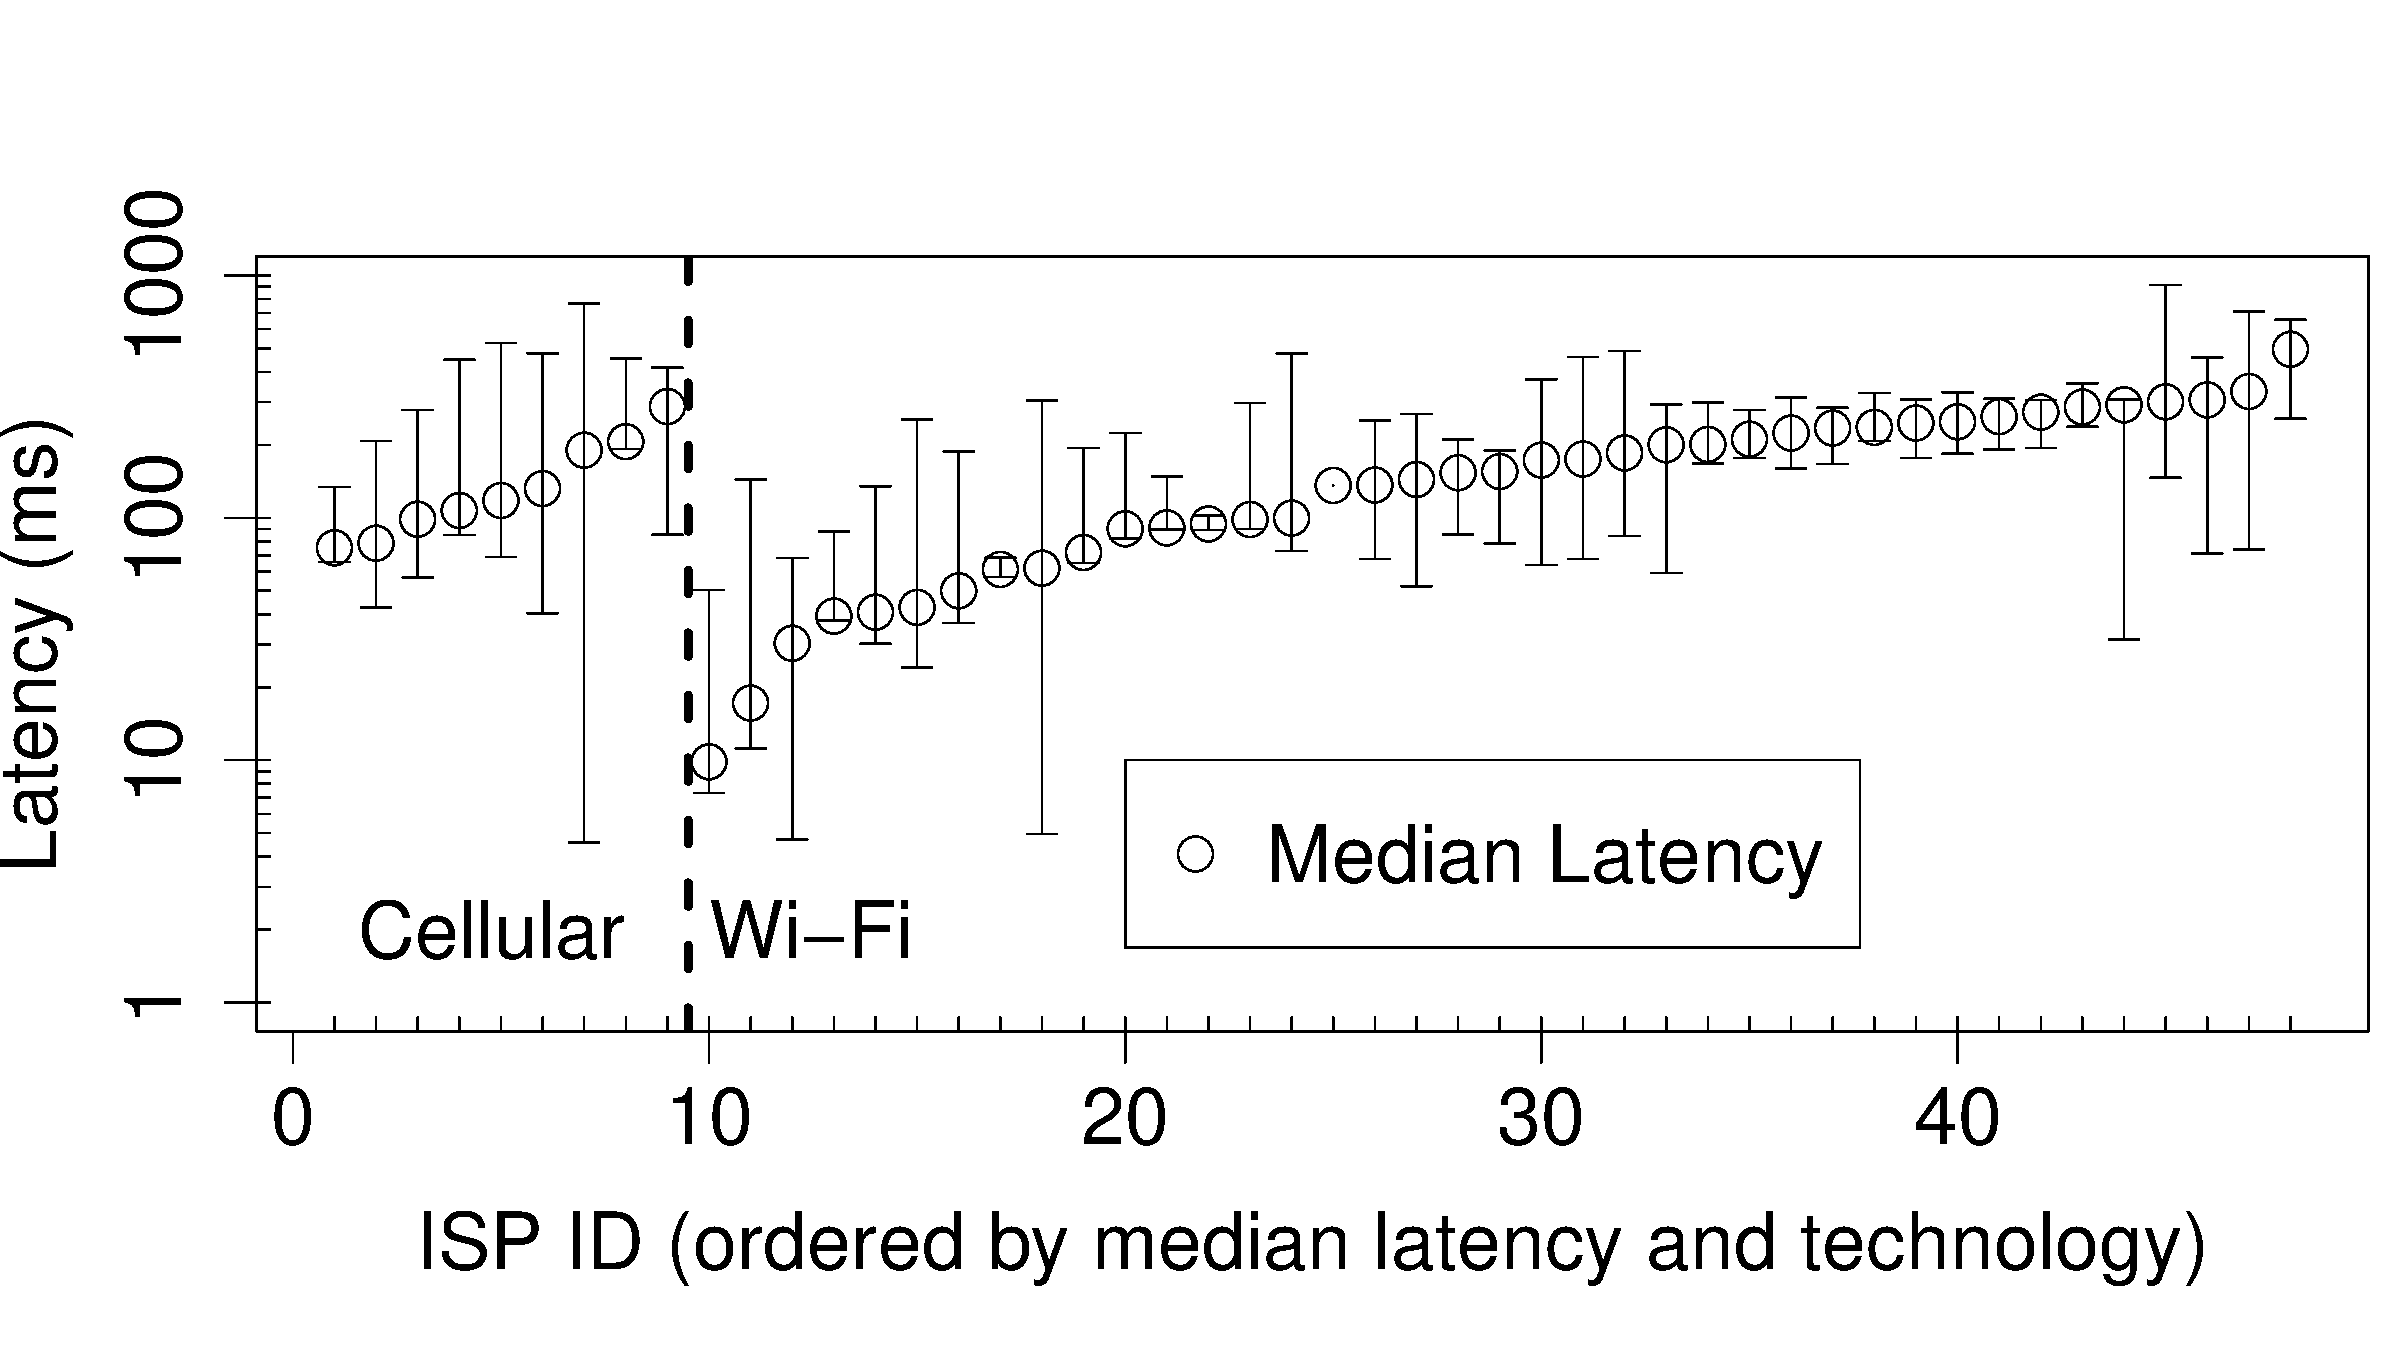
\includegraphics[width=\columnwidth]{plots/latency_isp_whisker.pdf}
\caption{One-way latency from VPN server to mobile devices. \emph{Connections from cellular ISPs suffer a higher delay compared to Wi-Fi ISPs. The delays from Cellular ISPs is comparable to connecting from a Wi-Fi ISP in another country. Error bars indicate the 91st and 9th percentile}.}
\label{fig:latency-across-isps}
\end{figure}


\begin{figure}[t]
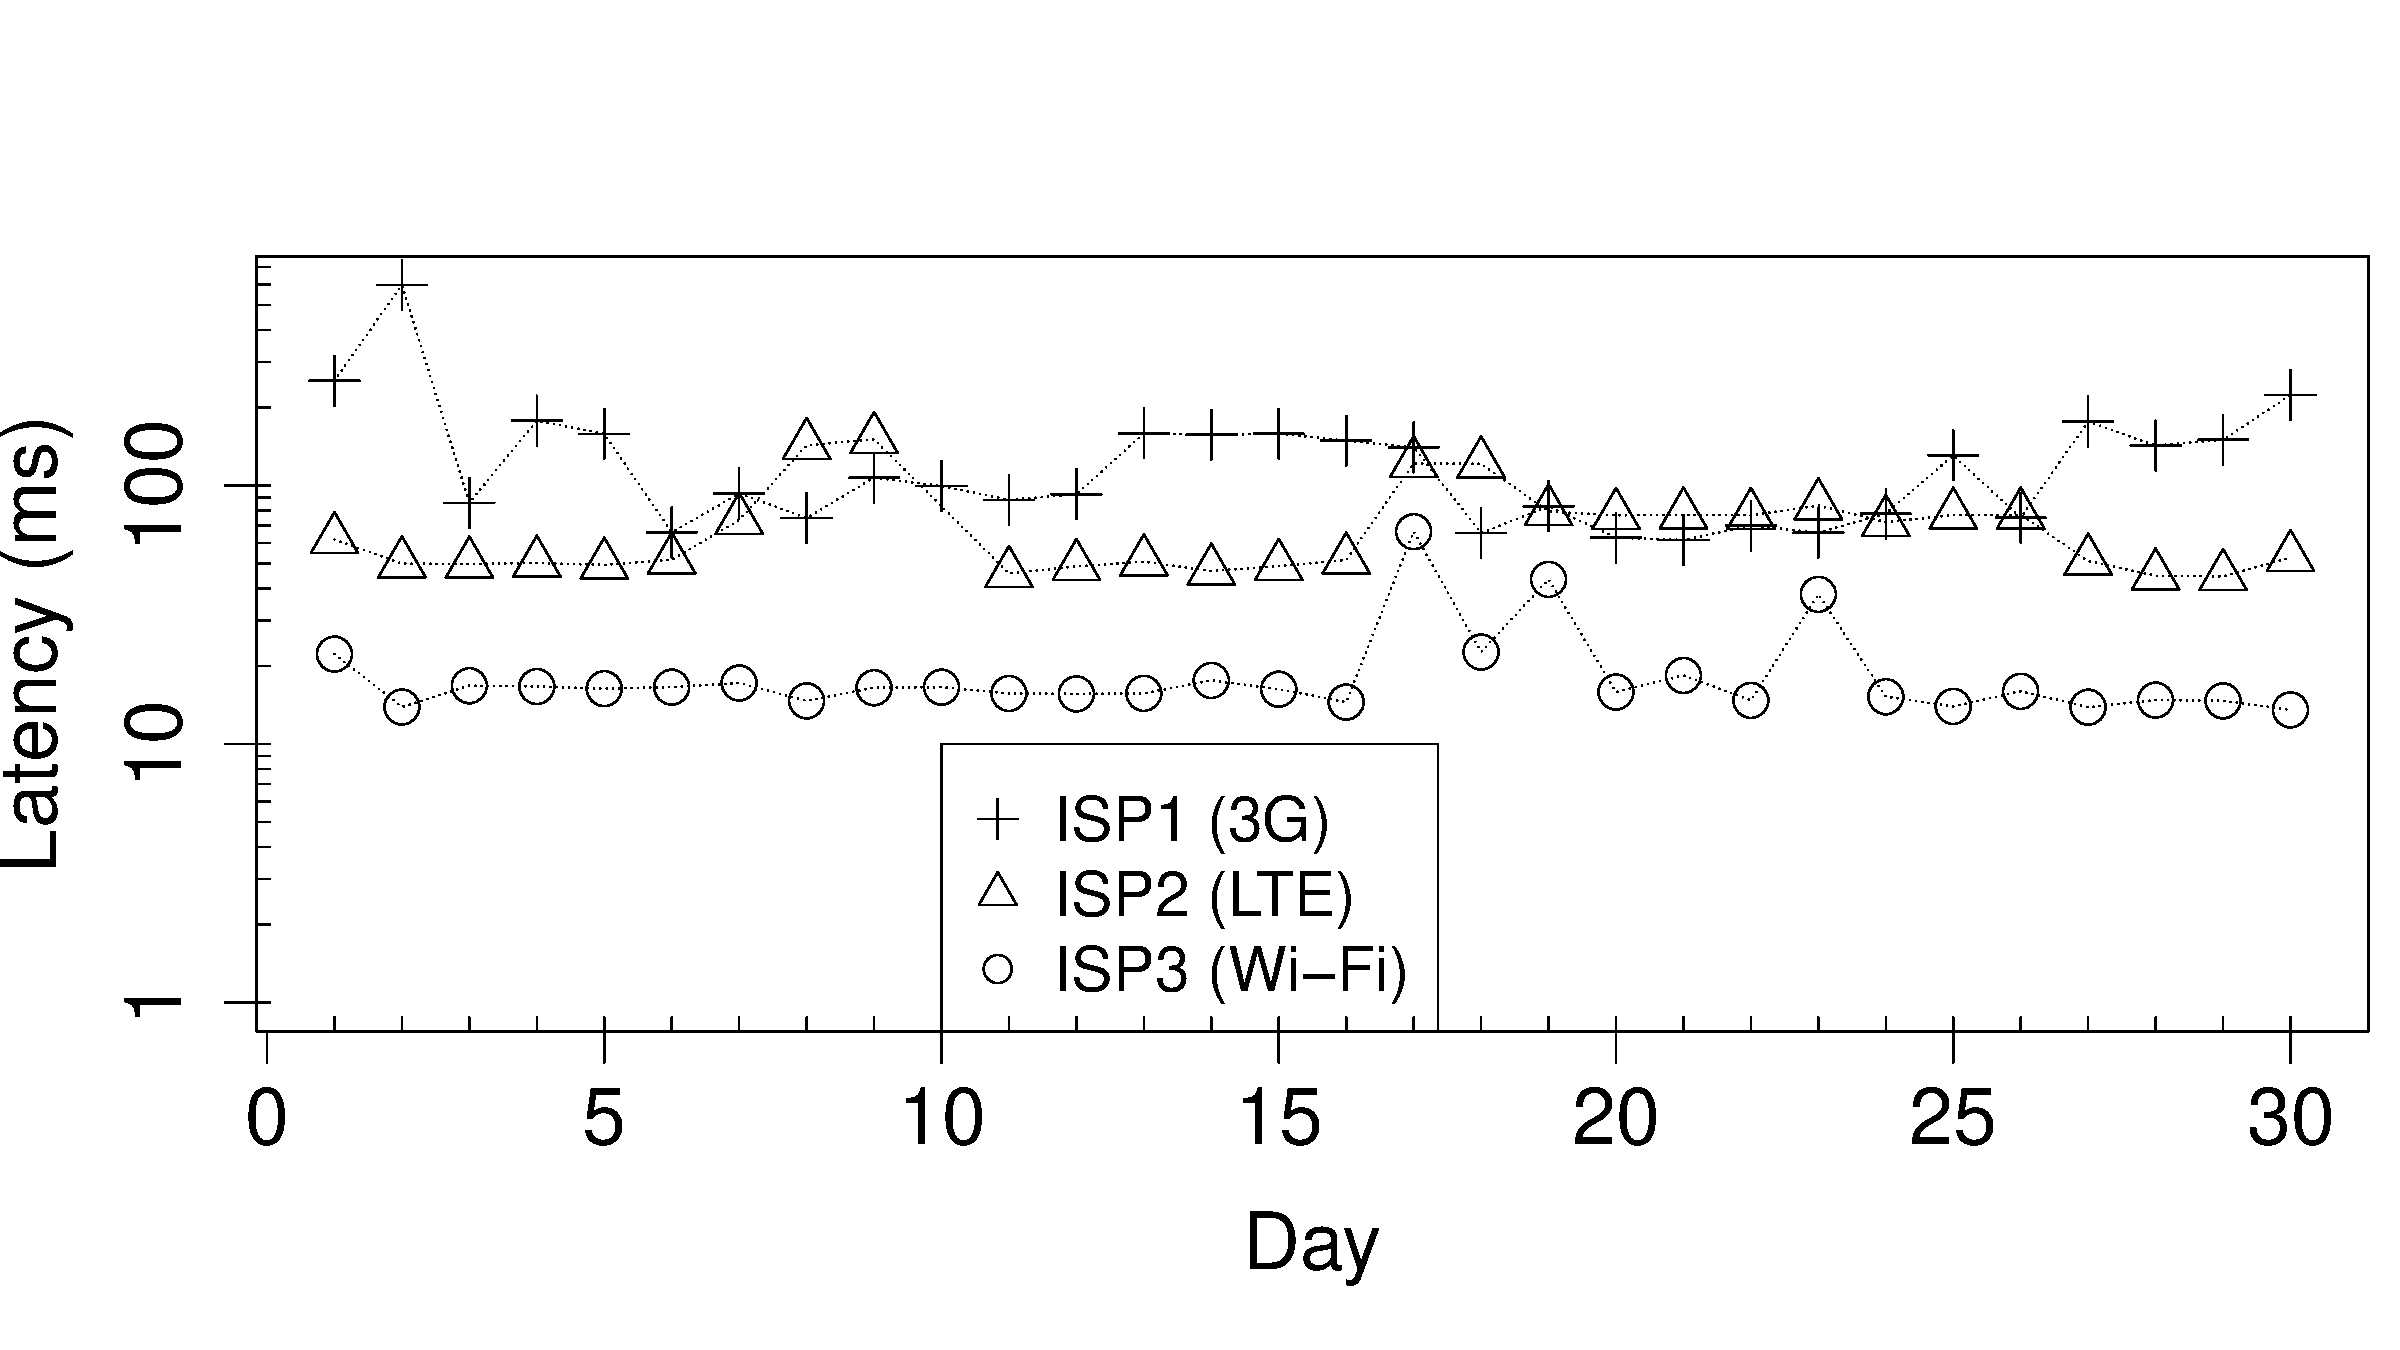
\includegraphics[width=\columnwidth]{plots/compare_isp_latency.pdf}
\caption{Comparison of ISPs that serve the same user during a 30 day time period. \emph{The LTE service provider has a smaller latency to the 3G provider. The smallest latency is observed by in the home Wi-Fi network.}}
\label{fig:compare-isp-latency}
\end{figure}

\begin{figure}[t]
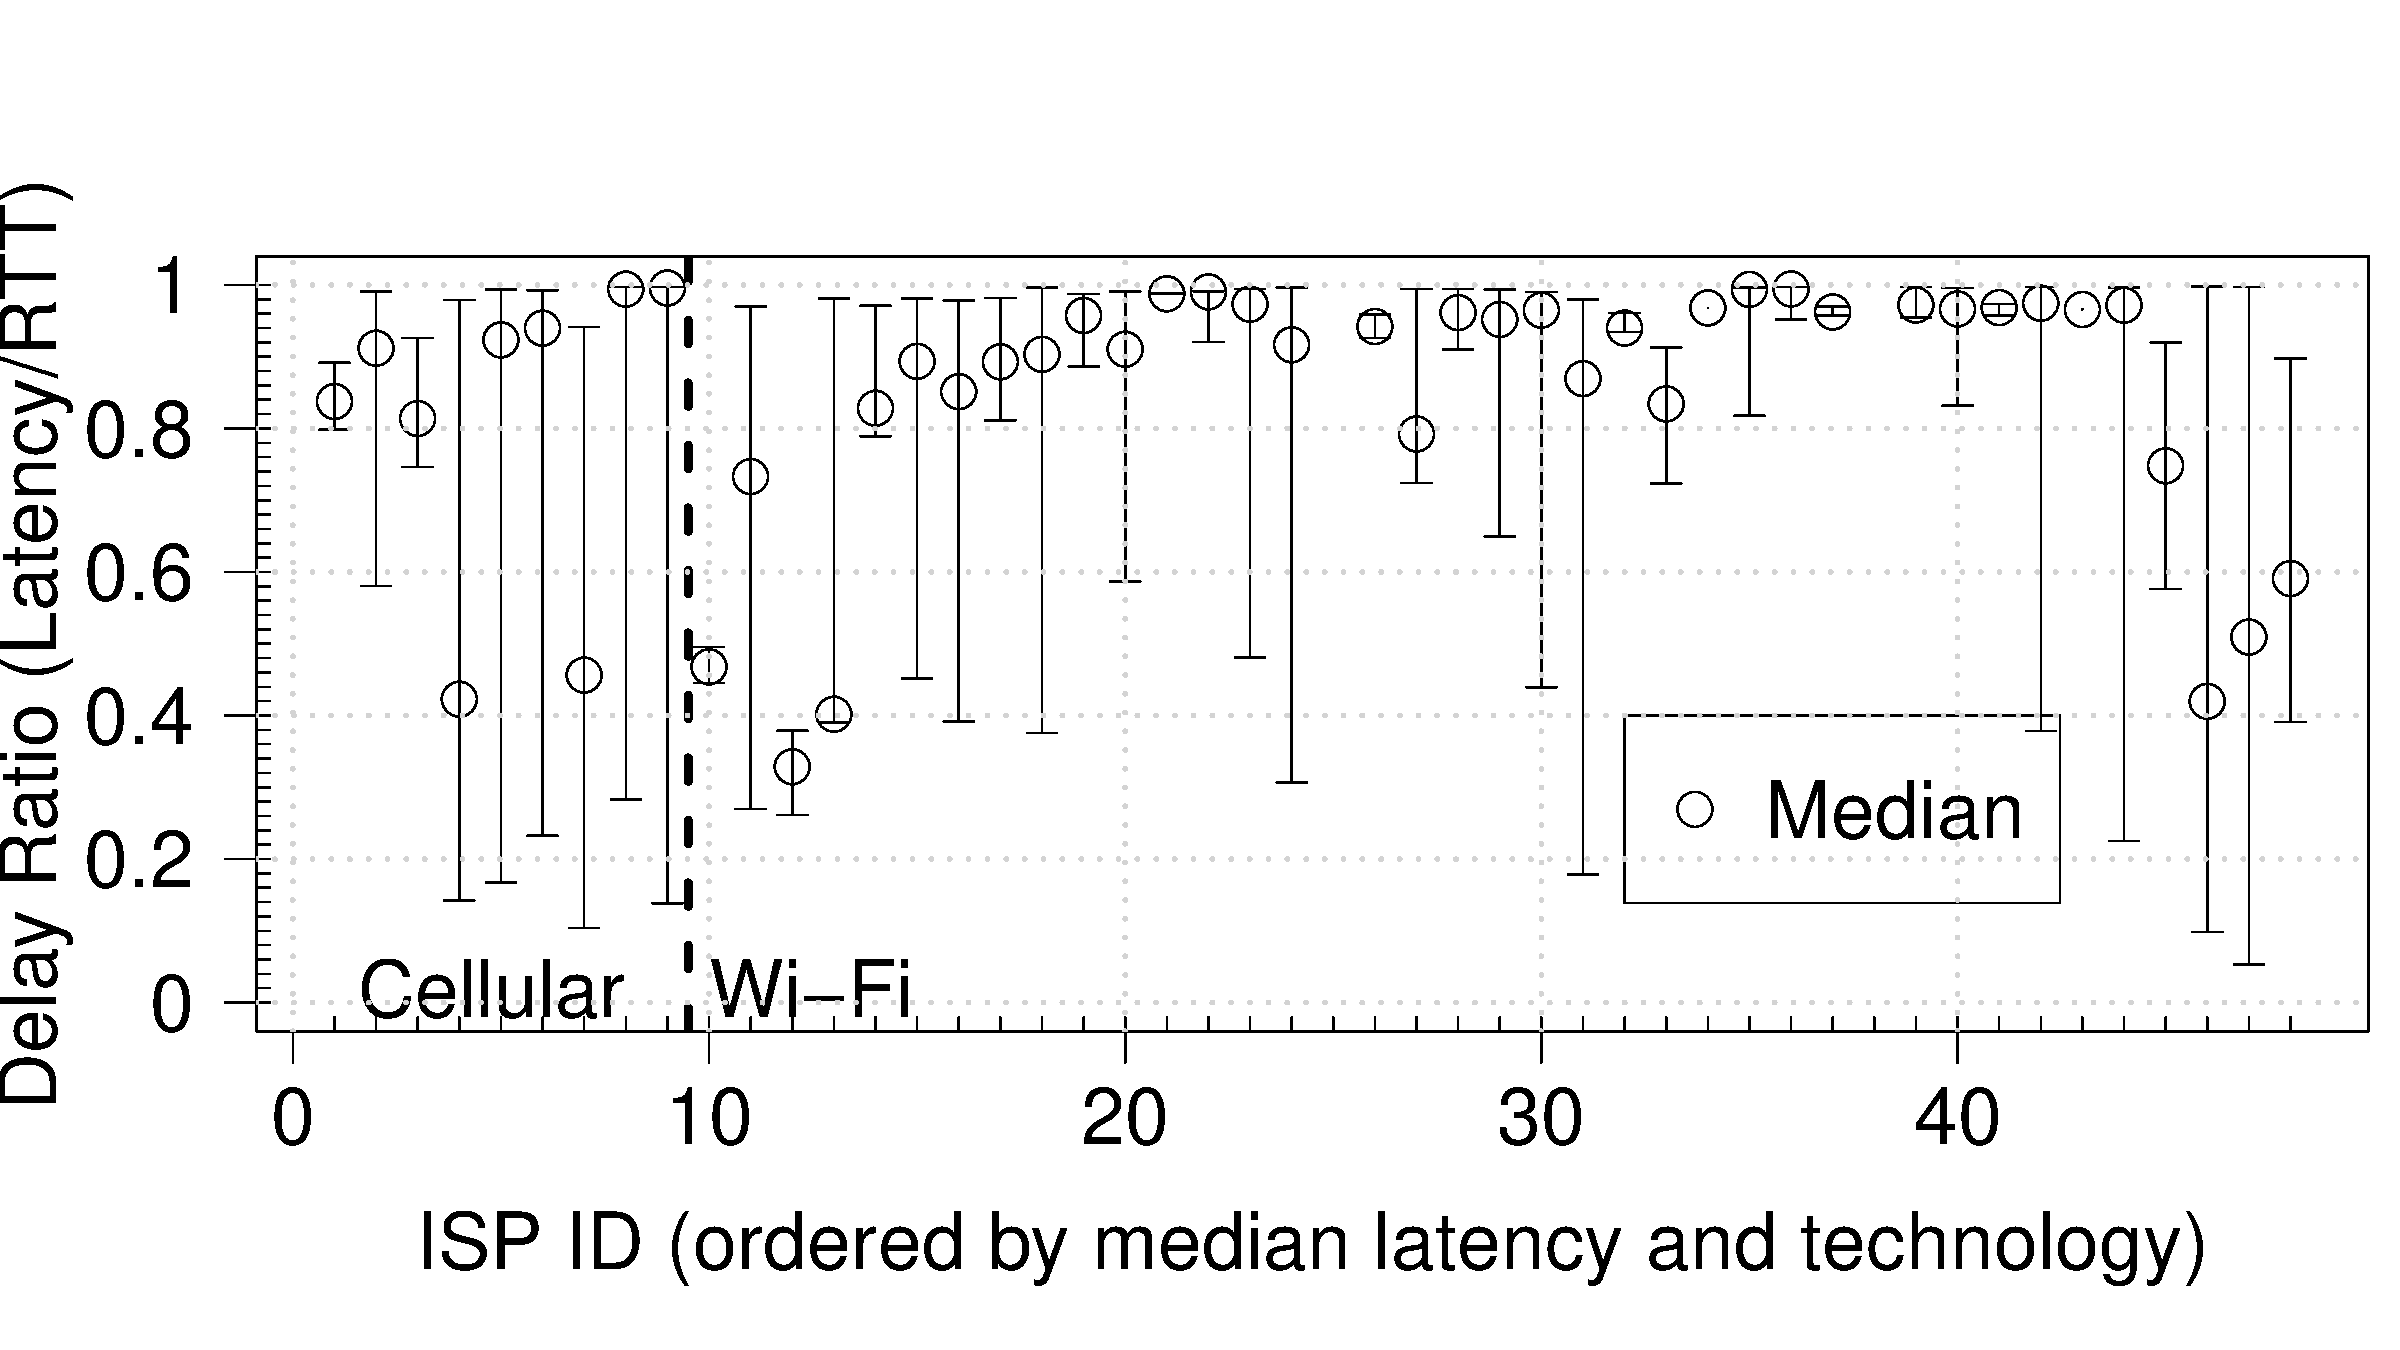
\includegraphics[width=\columnwidth]{plots/delay_ratio_isp_whisker.pdf}
\caption{Latency as a fraction of the round trip time to contact google services. \emph{In 35 ISPs of the 48 ISPs we observe that the latency of the mobile device to our server accounts for more than 90\% of the end-to-end round trip time. Error bars indicate the 91st and 9th percentile.}}
\label{fig:compare-delay-ratio}
\end{figure}

\begin{figure}[t]
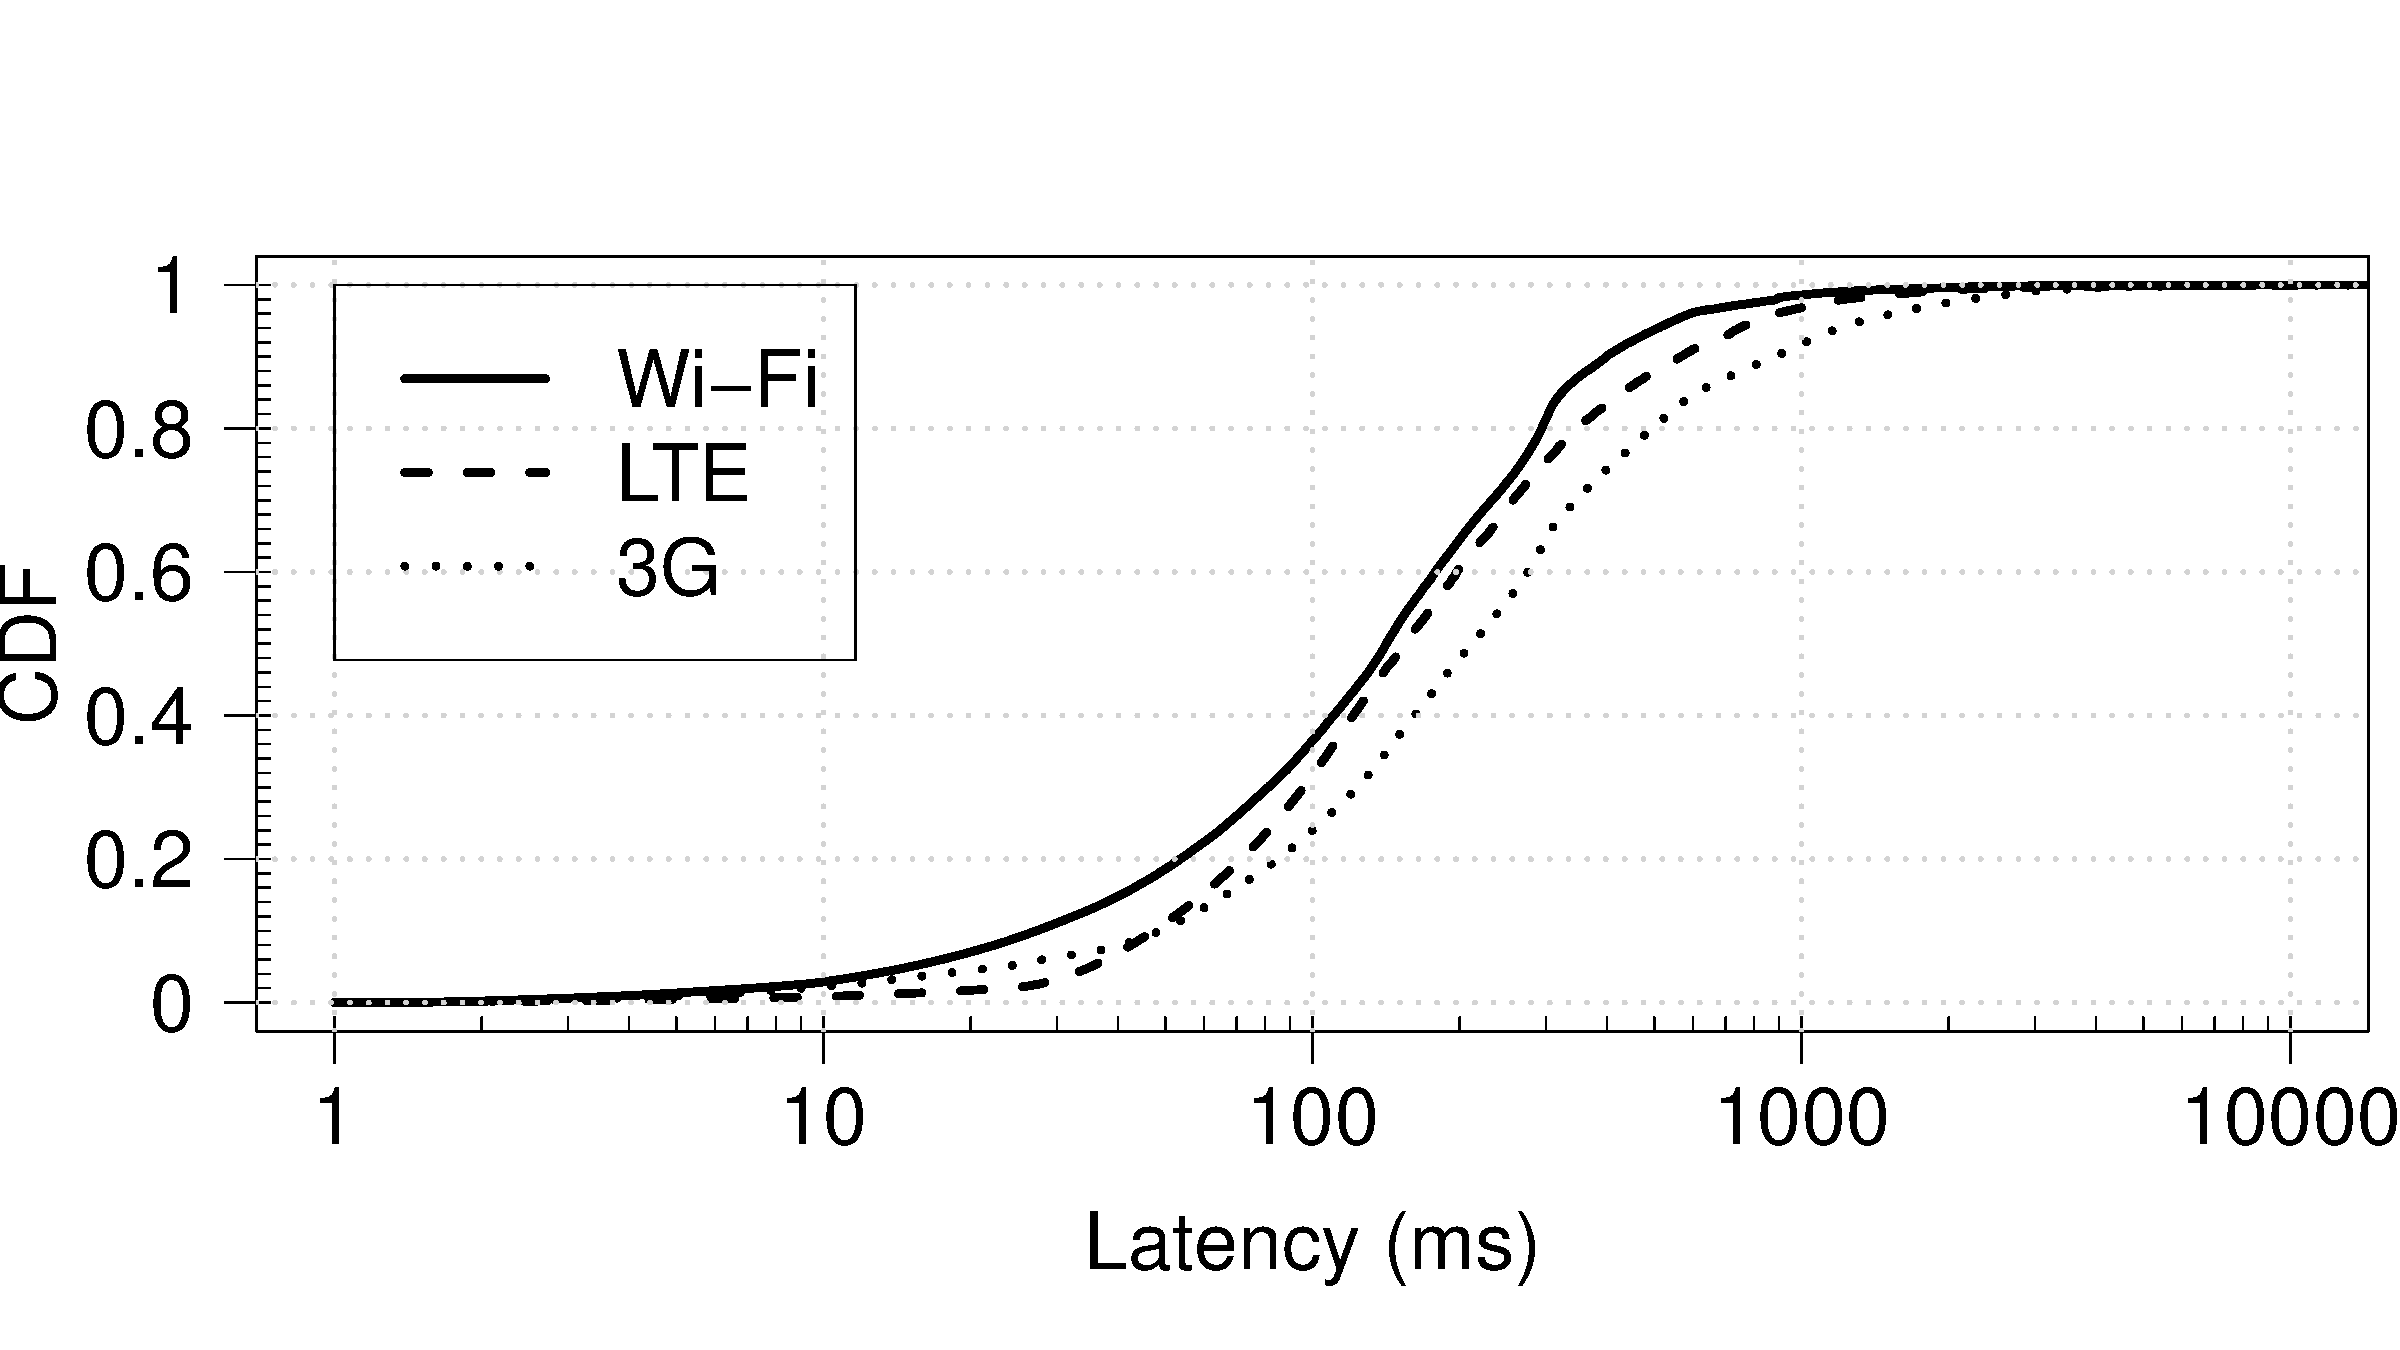
\includegraphics[width=\columnwidth]{plots/distrib_latency_technology.pdf}
\caption{Distribution of latency over cellular and \wifi ISPs. \emph{The distribution of latency observed when using LTE in the wild is similar to that observed for \wifi}.}
\label{fig:compare-delay-ratio}
\end{figure}

\begin{figure}[t]
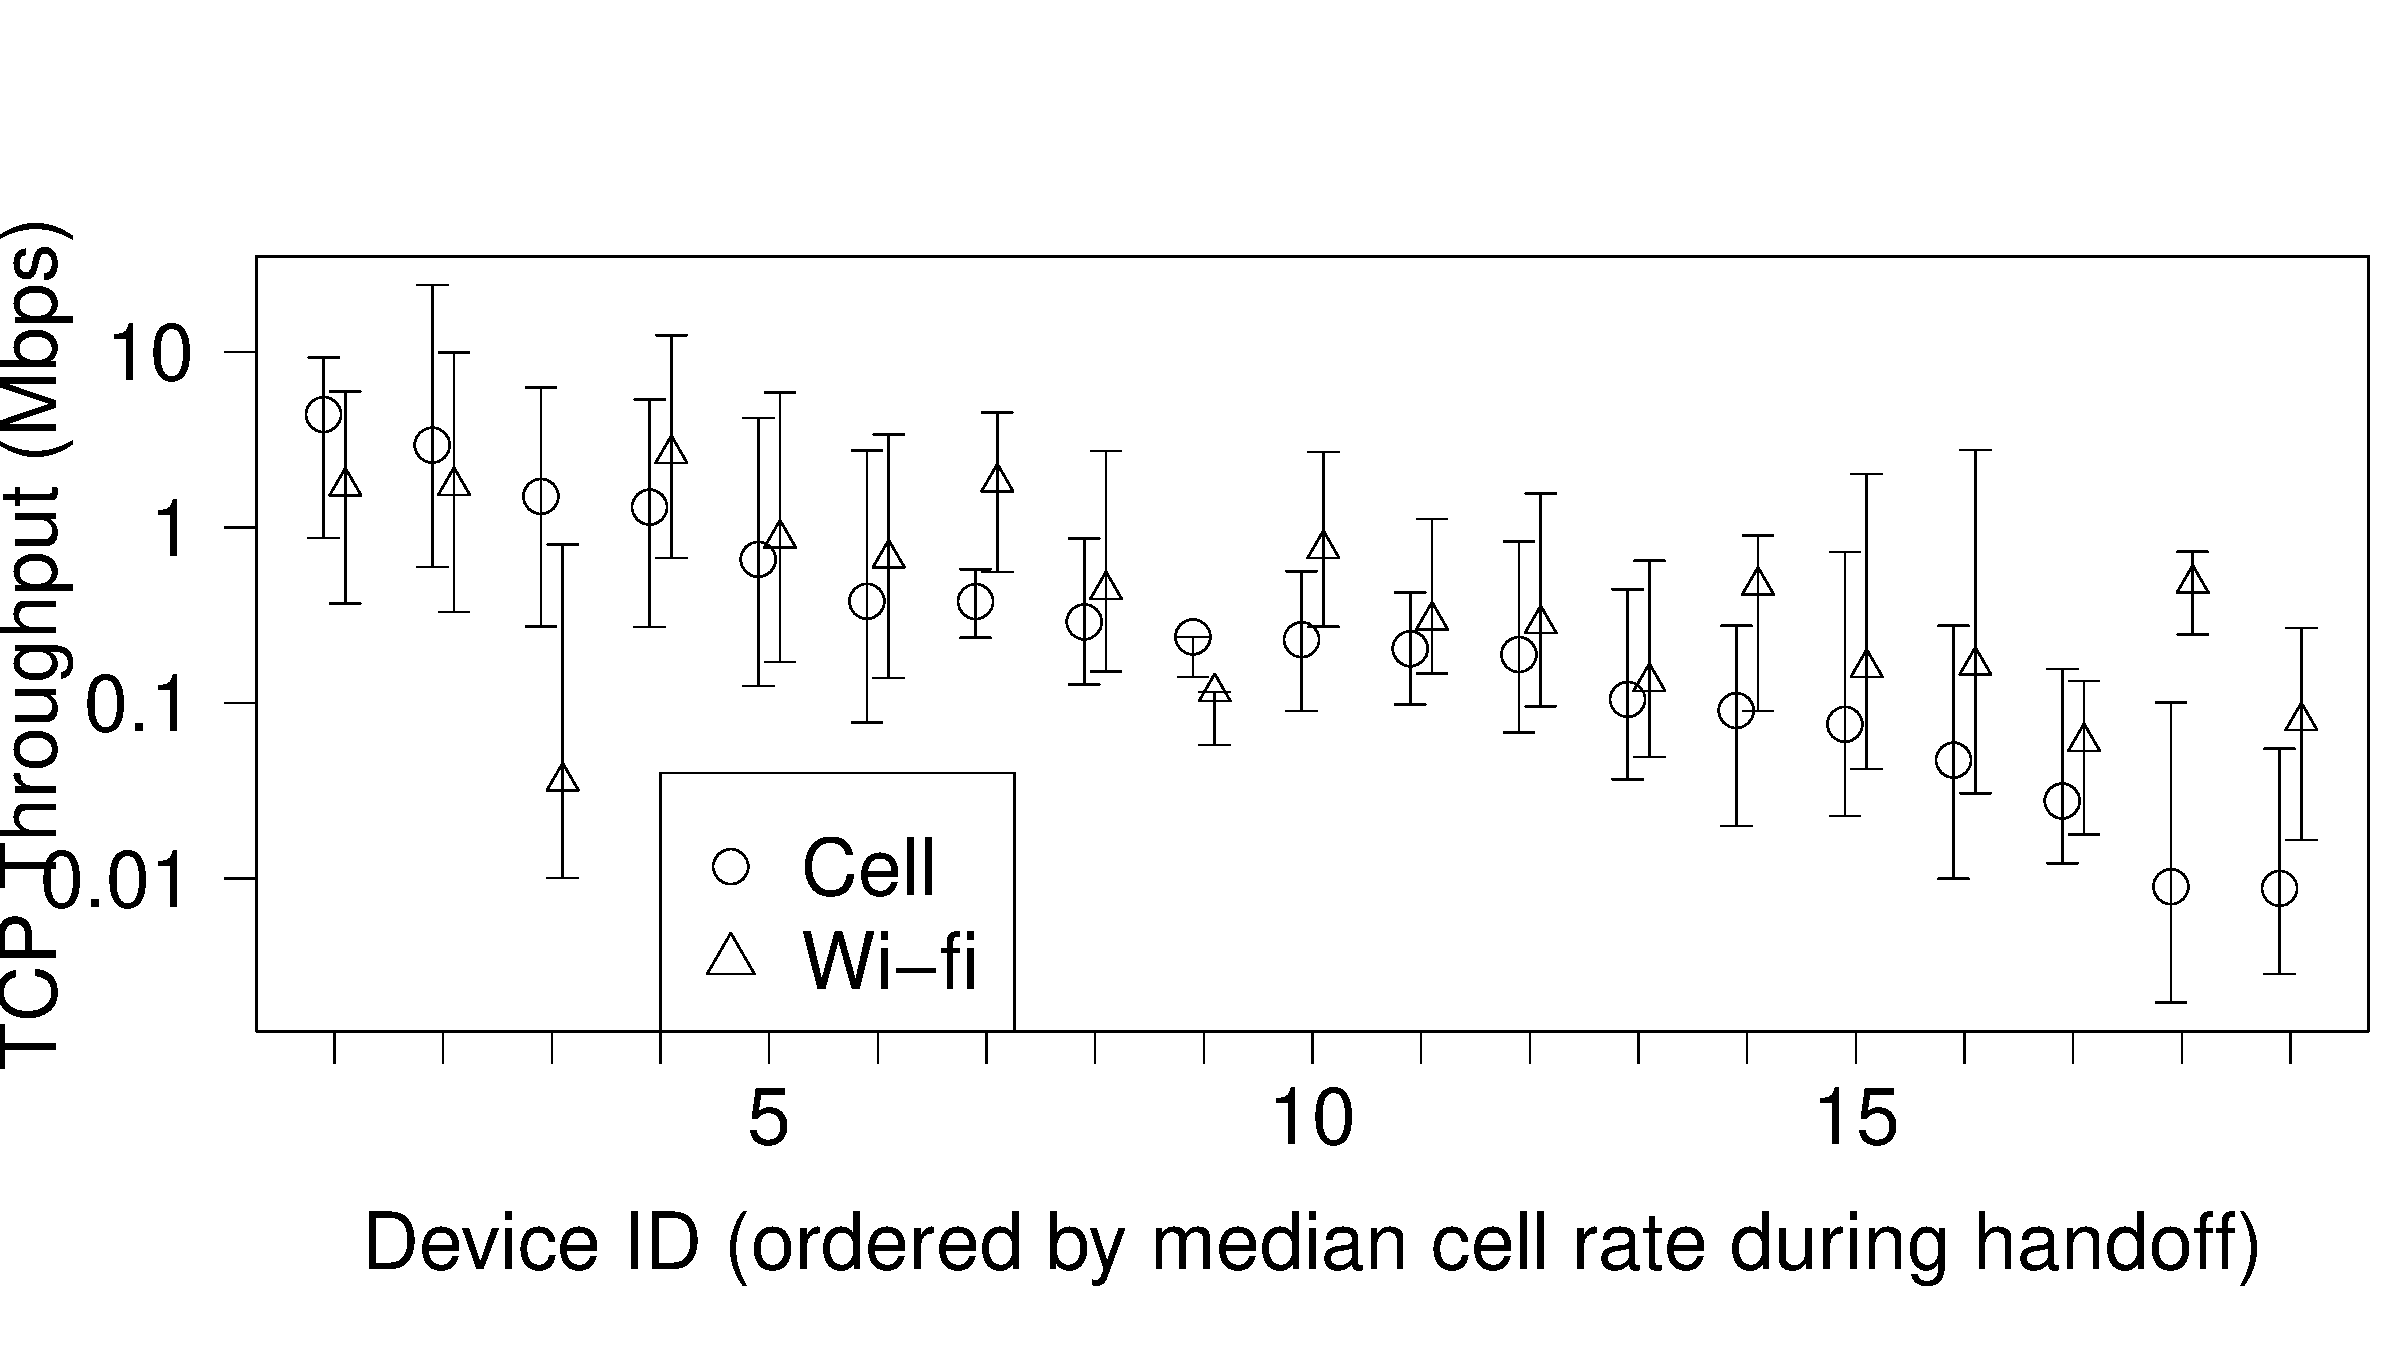
\includegraphics[width=\columnwidth]{plots/handoff_rates.pdf}
\caption{TCP Throughput observed during the hour of the handoff. \emph{The three users that have LTE connections observed a better TCP throughput over LTE in comparison to \wifi in the hour of the handoff. Error bars indicate the 91st and 9th percentile}.}
\label{fig:compare-handoff}
\end{figure}




\tbd{We performed a traceroute from our server to the egress link and found }





%\section{Related Work}
\label{sec:related}

The network behavior of mobile systems has implications for battery life, 
data-plan consumption, privacy, security and performance, among others. 
When attempting to characterize this behavior, researchers face a number 
of trade-offs: compromising network coverage (limiting the number and type of ISPs measured), 
portability (limiting the device OSes) and/or deployability (limiting subscriber coverage).
\platname compromises 
none of these, enabling comprehensive measurements across carriers, devices and access 
technologies. Table~\ref{tab:relatedCompare} puts our approach in context with previous 
approaches for measuring the network behavior of mobile systems. 

\begin{table*}[t]
\begin{center}
{\footnotesize
\begin{tabular}{|l|l|l|l|l|}
\hline
 & \textbf{Network Coverage} &  \textbf{Portability} &  \textbf{Deployment model} &   \textbf{Meas. Type}  \\ \hline
AT\&T/Telefonica study~\cite{vallina-rod:ads,gerber:passivespeed} & Single carrier & All OSes & Instrument cell infrastructure & Passive \\ \hline
WiFi study~\cite{chen:wifi} & Single WiFi network & All OSes & Instrument WiFi network & Passive \\ \hline
PhoneLab/TaintDroid~\cite{enck:taintdroid} & Multiple networks & Android & Install custom OS & Active/Passive \\ \hline
MobiPerf~\cite{wang:middleboxes}/SpeedTest~\cite{sommers:cellwifi} & Multiple networks & Android & Install App & Active \\ \hline
\platname & Any network & Android / iOS & VPN configuration & Passive \\ \hline
\end{tabular} }
\end{center}
\label{tab:relatedCompare}
\caption{Comparison of alternative measurement approaches. \platname is the first approach to cover all access networks and most device OSes, capturing 
network traffic passively and with low overhead via VPN proxying.}
\end{table*}%

Traces from mobile devices can inform a number of interesting analyses. Previous work 
uses custom OSes to investigate how devices waste energy~\cite{pathak:eprof}, network bandwidth and 
leak private information~\cite{enck:taintdroid,hornyack:appfence}. Similarly, AppInsight~\cite{ravindranath:appinsight} and PiOS~\cite{egele:pios} can inform 
app performance through binary instrumentation and/or static analysis. In this work, we explore the opportunity to use network traces 
alone to reveal these cases without requiring any OS or app modifications.

Network traces from inside carrier networks provide a detailed view for large numbers 
of subscribes. For example, Vallina-Rodriguez~\etal~\cite{vallina-rod:ads} uses this approach to characterize performance and 
the impact of advertising. Gerber \etal~\cite{gerber:passivespeed} similarly use this approach to 
estimate network performance for mobile devices.  \cite{maier:mobtraffic} \cite{chen:wifi}
Similar to these approaches, \platname provides continuous passive monitoring of mobile network 
traffic; however, \platname is the first to do so across all networks to which a device connects.

Last, active measurements~\cite{wang:middleboxes,sommers:cellwifi} allow researchers to understand network topologies and instantaneous 
performance at the cost of additional, synthetic traffic for probing. In contrast, \platname uses 
passive measurements to characterize the traffic that devices
naturally generate.

%%% Local Variables: 
%%% mode: latex
%%% TeX-master: "main.tex"
%%% End: 


Bro port based classification of HTTP, SSL, other, and so on. 


\section{Classification of Application}

\platname enables us to monitor the data being exchanged by the mobile device. 
However, it does not provide any details of the source of the data. 
We use the following technique to estimate the source of the mobile data traffic. 
In \ref{tab:summaryIOSAndroidTraffic} and \ref{tab:summaryWifiCellularTraffic} we observe that TCP is responsible for the majority of the traffic volume from iOS and Android devices regardless of the access technology used. 
We therefore focus on associating TCP flows to the applications for our analysis. 
From our analysis we were able to classify \tbdv{x\%} of the TCP traffic volume and \tbdv{y\%} of the TCP flows to the applications.

\subsection{Methodology}

\subsection{Results}

User Agent based classification
flows per user with a blank user agent. 
flows per user with a default user agent 
flows with application in user agent


SSL certificate based classification
flows to dedicated hosts
flows to cdns

\subsection{Discussion}

\section{Specific application behavior}


\section{Ads and Analytics}

Ads and Analytic sites have received considerable attention.
The reason for the attention being the intrusiveness exhibited by the ads and analytics sites in tracking personal information. 
\cite{vallina-rod:ads} show that \tbdv{ } of data traffic volume observed from a Cellular ISP is because of mobile ads. 
In our traces we use the classification of \cite{vallina-rod:ads} and \cite{YoyoAds} to classify flows as ads flows. 



\section{Discussion on Platform}

IPv6 support of VPNs

ISP support of VPNs. One ISP blocked VPN access. 

Open source ??

Releasing datasets ??


